\chapter{Dynamic Time Lag Regression: Predicting What \& When}\label{chapter:pdt}

\section{Introduction}\label{sec:intro}
A significant body of work in machine learning concerns the modeling of spatio-temporal phenomena \citep{SurveyST,NIPSForecasting18}, 
ranging from markets \citep{Pedreschi} to weather forecasting \citep{Horvitz}.
This paper focuses on the problem of modeling the temporal dependency between two time series, 
where the latter one is {\em caused} by the former one \citep{Granger} with a non-stationary time delay. 

The motivating application domain is that of space weather. The sun, a perennial source of charged energetic particles, 
is at the origin of geomagnetic phenomena within the sun-earth system. Specifically, the sun ejects 
charged particles into the surrounding space in all directions and some of these particle clouds, a.k.a. solar wind, 
reach the earth vicinity. High speed solar wind is a major threat for the modern world, causing severe damages to 
e.g., satellites, telecommunication infrastructures, under sea pipelines, among others.
\footnote{The adverse impact of space weather is estimated to cost 200 to 400 millions per year, 
but can sporadically lead to much larger losses.} 

A key prediction task thus is to forecast the speed of the \emph{solar wind} in the vicinity of the Earth 
\citep{doi:10.1002/jgra.50429,doi:10.1029/2009SW000542}, sufficiently early to emit an alarm and be able to prevent 
the damages to the best possible extent. Formally the goal is to model the dependency between heliospheric 
observations (available at light speed), referred to as {\em cause series}, and the solar wind speed series recorded at the 
Lagrangian point $L_1$ (distant from the Earth by 1.5 million kilometers), referred to as {\em effect series}. The 
key difficulty is that the time lag between an input and its effect, the solar wind recorded at $L_1$, varies from circa 2 to 5 days
depending on, among many factors, the initial direction of emitted particles and their energy. Would the lag be constant, the solar wind 
prediction problem would boil down to a mainstream regression problem. The challenge here is to predict, from the solar image $x(t)$ at time $t$ the 
value $y(t+\tau)$ of the solar wind speed reaching the earth at time $t+\tau$ where both the value $y(t+\tau)$ and the time lag $\tau$ depend on $x(t)$.

To our knowledge the regression problem of predicting both {\em what} the effect is and {\em when} the effect is observed constitutes a new ML problem, 
that we called {\em Dynamic TimeLag Regression} (\XX). Indeed, the modeling of dependencies among financial 
time series has been intensively tackled (see e.g. \citet{ZHOU2006195}). When considering varying time lag, 
many approaches rely on dynamic time warping (DTW) \citep{SakoeShiba1978}. For instance, DTW is used in 
\citet{SignalDiffusion}, taking a Bayesian approach to achieve the temporal alignment of both series under some restricting assumptions 
(considering slowly varying time lags and linear relationships between the cause and effect time series). More generally, 
the use of DTW in time series analysis relies on simplifying assumptions on the cause and effect series 
(same dimensionality and structure) and build upon available cost 
matrices for the temporal alignment. 

This paper focuses on the \XX\ regression problem and the identification of varying time-lag phenomena involving stochastic dependencies of
arbitrary complexity. The originality of the proposed approach compared to the state of the art 
in DTW series alignment is threefold. Firstly, the cause and effect series are of different dimensionality. 
While the effect series is scalar, the cause series can be high-dimensional (e.g. images). %, vectors, etc). 
Secondly, the relationship 
between the cause and the effect series can be non-linear (the {\em what} model). Thirdly, the time lag phenomenon 
(the {\em when} model) can be non smooth (as opposed to e.g. \citet{ZHOU2006195}).

The Bayesian approach proposed to tackle the \XX\ regression problem and the associated learning 
equations are described in section \ref{sec-formulation}, followed by a stability analysis and a 
proof of consistency (section \ref{sec-theory}). The algorithm is detailed in section \ref{sec:model}. 
The experimental setting used to validate the approach is presented in section \ref{sec:exp}, and 
the proofs of concept of the approach are discussed in section \ref{sec:proofconcept}

\paragraph{Notations.}
Given two time series, the cause series $x(t)$ and the observed effect series $y(t)$, the sought model 
consists of a mapping $f(.)$ which maps each input pattern $x(t)$ to an output $y(t')$, and a 
mapping $g(.)$ which maps $x(t)$ onto the time delay $t'-t$ between the input and output patterns:

\begin{align}
y(t + \tau(t)) & = f[x(t)]\label{eq:pb1}\\
\tau(t) & = g[x(t)]\label{eq:pb2} 
\end{align}
with
\[
f: \mathcal{X}  \rightarrow \mathbb{R},\qquad\text{and}\qquad
g: \mathcal{X}  \rightarrow \mathbb{R}^{+},
\]
where $t \in \mathbb{R}^{+}$ represents the continuous temporal domain. The input signal 
$x(t)\in \mathcal{X}$ is possibly high dimensional and contains the hidden cause to 
the effect $y(t)\in\mathbb{R}$ which is considered as a scalar in this paper. 
$\tau(t)\in \mathbb{R}^+$ represents the time delay between inputs and outputs.
Vectors are written using bold fonts.

\section{Probabilistic Dynamically Delayed Regression}\label{sec-formulation}
As said, Eqs \ref{eq:pb1}-\ref{eq:pb2} define a regression problem that differs from standard regression along two lines. 
Firstly, the time lag $\tau(t)$ is non-stationary as it depends on $x(t)$.  
Secondly, $\tau(t)$ is unknown, i.e. it 
is not recorded explicitly in the training data as is typically the case in the space weather context. 
\subsection{Assumptions}
For the sake of the model identifiability and computational stability, the delay function $\phi(t) = t + \tau(t)$ is assumed to be sufficiently regular w.r.t. $t$. Formally,  $\phi(.)$ is assumed to be continuous. % and \emph{bijective}. I remove this, which is not consistent with the model

For some authors  \citep{ZHOU2006195} the monotonicity of $\phi(.)$ is additionally required and enforced using constraints:   $$\phi(t_1) \leq \phi(t_2), \forall t_1 \leq t_2$$
However, this assumption will not be retained in the following as it does not hold in the space weather domain (e.g. fast moving 
solar wind can reach the Earth before slow moving solar wind which departed before it). 

\subsection{Probabilistic Dynamic Time-Lag regression}
For practical reasons, cause and effect series are sampled with a constant rate $\delta t$, and respectively noted ${x_m}$ and ${y_m}$ in the following. Accordingly, mapping $g$ might be sought as a discrete time lag, where the delay between cause $x_m$ and effect $y_{m+g(x_m)}$ ranges in a finite set $T = [\tau_{min}, \ldots, \tau_{max}]$, with  $\tau_{min}$ and  $\tau_{max}$ defined from prior knowledge, e.g. space weather theory. 

The unavoidable error due to the discretization of the continuous time lag is mitigated along a probabilistic model, associating to each cause $x$, a set of independent predictors $\{\hat y_i(x),i=$ in $T\}$ and a probability distribution $\hat p(x)$ on $T$ estimating the probability of delay of the effects of $x$. Overall, the \XX\ solution is sought as a probability distribution conditioned on cause $x$, mixture of Gaussians centered on the predictors $\hat y_i(x)$, where the mixture weights are defined from $\hat p(x)$. More formally, letting ${\bf y}_m$ denote the vector of random variables $y_{m+i}, i$ in $T$, 
\begin{equation}\label{eq:py}
  P\bigl[{\bf y}_{m}\vert x_m=x\bigr] = \sum_{i \in T, \tau_i\in\{0,1\}}  \hat p\bigl(\tau_1,\ldots,\tau_n\vert x)
\prod_{i\in T} {\cal N}\bigl(\hat y_i(x),\sigma_i(\tau)\bigr)
\end{equation}
Two simplifications are made for the sake of the analysis. Firstly, the stochastic time lag is modelled as the set $\{\tau_i, i$ in $ T\}$ of binary 
latent variables, where $\tau_i$ indicates whether $x$ drives $y_i$ ($\tau_i=1$) or not ($\tau_i=0$). The assumption that every cause has a single effect is modelled by imposing:\footnote{Note however that the cause-effect correspondence might be many-to-one, with an effect depending on several causes.}
\begin{equation}\label{eq:cs1}
\sum_{i \in T} \tau_i = 1.
\end{equation}
From constraint~(\ref{eq:cs1}), probability distribution $\hat p(x)$ thus is sought as a set of $\hat p_i(x)$ for $i$ in $T$, summing to 1, such that $\hat p_i(x)$ stands for the 
probability of the effect of $x_m=x$ to occur with delay $i$ in $T$. \\
The second simplifying assumption is that the variance $\sigma_i^2({\bf \tau})$ of predictor $\hat h_i$ does not depend on $x$, by setting:
\[
\sigma_i({\bf \tau})^{-2} = \Bigl(1+\sum_j\alpha_{ij} \tau_j\Bigr)\sigma^{-2},
\]
with $\sigma^2$ a default variance and $\alpha_{ij}\ge 0$ a matrix of non-negative real parameters. 
The fact that $x$ can influence $y_i$ through predictor $\hat y_i(x)$ even when $\tau_i=0$ reflects an indirect
influence due to the auto-correlation of the $y$ series. This influence comes with a higher variance, enforced by making 
$\alpha_{ij}$ a decreasing function of $\vert i-j\vert$. More generally, a large value of $\alpha_{ii}$ compared to $\alpha_{ij}$ for $i\ne j$ corresponds to a small auto-correlation time of the effect series. 


\subsection{Learning criterion}
The joint distribution is classically learned by maximizing the log likelihood of the data, that can be computed 
in closed form as (please see supplementary material appendix \ref{app:LL} for the details of the calculation): 
\begin{equation}\label{eq:LL}
{\cal L}\bigl[ {\bf x, y};\hat {\bf y},\hp,\sigma,{\bf \alpha}] = -\vert T\vert\log(\sigma)-\frac{1}{n_m}\sum_m\Bigl[\sum_{i \in T}\frac{1}{2\sigma^2}\bigl(
y_{m+i}-\hat y_i(x_m)\bigr)^2
-\log\bigl(Z_m(\hat {\bf y},\hp,\sigma,{\bf \alpha})\bigr)\Bigr],
\end{equation}
with $n_m$ the number of data points and partition term $Z_m$ given as:
\[
Z_m(\hat {\bf y},\hp,\sigma,{\bf \alpha}) = \sum_{i \in T}\hat p_i(x_m)\exp\Bigl(-\frac{1}{2\sigma^2}\sum_{j\in T}\alpha_{ji}\bigl(y_{m+j}-\hat y_j(x_m)\bigr)^2+\frac{1}{2}\sum_{j\in T}\log(1+\alpha_{ji})\Bigr)
\]
For notational simplicity, the data index $m$ is omitted in the following and the empirical averaging on the data is noted ${\mathbb E}_{data}$.
The hyper-parameters $\sigma$ and matrix $\alpha$ of the model are obtained by optimizing  ${\cal L}$:
\begin{equation}\label{eq:var}
\frac{\sigma^2}{1+\alpha_{ij}} = \frac{{\mathbb E}_{data}\bigl[\bigl(y_i-\hat y_i(x)\bigr)^2q_j(x,{\bf y})\bigr]}
{{\mathbb E}_{data}\bigl[q_j(x,{\bf y})\bigr]},
\end{equation}
%%%% I change $p_i(x,y)$$ for $q: not the same letter with different arguments.
with the probability $q_i(x,{\bf y}) = P(\tau_i=1\vert x,{\bf y})$ defined as
\begin{equation}\label{eq:hatpi}
q_i(x,{\bf y}) = \frac{1}{Z(\hat {\bf y},\hp,\sigma,{\bf \alpha})}\hat p_i(x)\exp\Bigl(-\frac{1}{2\sigma^2}\sum_{j\in T}\alpha_{ji}\bigl(y_j-\hat y_j(x)\bigr)^2+\frac{1}{2}\sum_{j\in T}\log(1+\alpha_{ji})\Bigr)
\end{equation}
In addition the optimal $\hat {\bf y}$ and $\hp$ reads:%(see appendix~\ref{app:LL})
\begin{align}
\hat y_i(x) &= \frac{{\mathbb E}_{data}\Bigl[y_i\bigl(1+\sum_{j\in T}\alpha_{ij}q_j(x,{\bf y})\bigr)\Big\vert x\Bigr]}
{{\mathbb E}_{data}\Bigl[1+\sum_{j\in T}\alpha_{ij}q_j(x,{\bf y})\Big\vert x\Bigr]}\label{eq:hyopt}\\[0.2cm]
\hat p_i(x) &= {\mathbb E}_{data}\Bigl[q_i(x,{\bf y})\Big\vert x \Bigr],\label{eq:tildep}
\end{align}
where the above conditional empirical averaging operates as an averaging over samples close to $x$.

These are implicit equations, since $q_i(x,{\bf y})$ depends on the parameters $\sigma^2$ and $\alpha_{ij}$, $\hat {\bf y}$ and $\hp$.
The proposed algorithm detailed in section \ref{sec:model} implements the saddle point method defined from Eqs (\ref{eq:var},\ref{eq:hatpi},\ref{eq:hyopt},\ref{eq:tildep}): alternatively,  hyper-parameters $\sigma$ and $\alpha_{ij}$ are updated from Eq. (\ref{eq:var}) based on the current $\hat y_i$ and $\hat p_i$; and predictors $\hat y_i$ and mixture weights  $\hat p_i$ are accordingly updated from respectively Eqs (\ref{eq:hyopt}) and (\ref{eq:tildep}). 

\section{Theoretical analysis}\label{sec-theory}
The proposed \XX\ approach is shown to be consistent and analyzed in the simple case  where $\alpha$ is a diagonal matrix ($\alpha_{ij} = \alpha\delta_{ij}$).

\subsection{Loss function and related optimal predictor}\label{sec:prop}
Let us assume that the hyper-parameters of the model have been identified together with predictors $\hat  y_i(x)$ and weights $\hat p_i(x)$. These are leveraged to achieve the prediction of the effect series. 
For any given input $x$, the sought eventual predictor is expressed as $(\hat y(x),\hat I(x))$ where $\hat I(x)$ is the predicted time lag %($= \arg\max_i \hat p_i(x)$) 
and $\hat y(x)$ the 
predicted value. The associated $L_2$ loss is: 
\begin{equation}\label{eq:orloss}
{\cal L}_2(\hat y,\hat I) = {\mathbb E}_{data}\Bigl[\bigl(y_{\hat I(x)}-\hat y(x)\bigr)^2\Bigr]. 
\end{equation}
Then it comes:
\begin{prop}\label{prop:opred}
With same notations as in Eq. (\ref{eq:py}), with $\alpha_{ij} = \alpha\delta_{ij},\ \alpha>0$, the optimal composite predictor 
$(y^\star,I^\star)$ is given by
\[
y^\star(x) = \hat y_{I^\star(x)}(x)\qquad\text{with}\qquad I^\star(x) = \argmax_{i} \bigl(\hat p_i(x)\bigr), 
\]
\end{prop}
\begin{proof}
In supplementary material, Appendix \ref{app:Hessian}.
\end{proof}

\subsection{Linear stability analysis}\label{sec:stability}
The saddle point Eqs (\ref{eq:var},\ref{eq:hatpi},\ref{eq:hyopt},\ref{eq:tildep}) admit among others a degenerate solution, corresponding 
to $\hat p_i(x) = 1/\vert T\vert$, $\alpha_{ij}=0$ for all pairs $(i,j)$, with $\sigma^2=\sigma_0^2$. Informally the model converges toward this degenerate trivial solution when there is not enough information to build specialized predictors $\hat y_i$. 

Let us denote $\Delta y_i^2(x)= \bigl(y_i-\hat y_i(x)\bigr)^2$ the square error made by predictor $\hat y_i$ for $x$, and 
\[
\sigma_0^2 = \frac{1}{|T|}{\mathbb E}_{data}\Bigl(\sum_{i \in T } \Delta y_i^2(x)\Bigr)
\]
the  MSE over the set of the predictors $\hat y_i$, $i \in T$. 

Let us investigate the conditions under which the degenerate solution may appear, by computing the Hessian of the log-likelihood and its eigenvalues. Under the simplifying assumption
\[
\alpha_{ij} = \alpha \delta_{ij},
\]
the model involves $2\vert T\vert+2$ parameters: $\alpha$, $r = \sigma^2/\sigma_0^2$, $\hat {\bf y}$ and $\hp$. After the computation of the Hessian (supplementary material, Appendix \ref{app:opred}) the system involves three key statistical quantities, two global ones:
\begin{align}
C_1[\p] &= \frac{1}{\sigma_0^2}{\mathbb E}_{data}\Bigl(\sum_{i \in T} q_i(x,{\bf y})\Delta y_i^2(x)\Bigr),\label{def:C1}\\[0.2cm]
C_2[\p] &= \frac{1}{\sigma_0^4}{\mathbb E}_{data}\Bigl[\sum_{i\in T}q_i(x,{\bf y})\Bigl(\Delta y_i^2(x)-\sum_{j \in T} q_j(x,{\bf y})\Delta y_j^2(x)\Bigr)^2\Bigr],\label{def:C2}
\end{align}
\[
\text{and a local one:}\qquad \vert {\bf u}(x)\vert^2 = \sum_{i\in T} C_{2+i}[x,\p]^2,
\]
where ${\bf u}(x)$ is a $\vert T\vert$-vector of components 
\[
C_{2+i}[x,\p] = \frac{1}{\sigma_0^2}{\mathbb E}_{data}
\Bigl[ q_i(x,{\bf y})\bigl(\Delta y_i^2(x)-\sum_{j \in T} q_j(x,{\bf y})\Delta y_j^2(x)\bigr)\Big\vert x \Bigr].
\]
Up to a constant, $C_1$ represents the covariance between the latent variables $\{\tau_i\}$ and the normalized predictor errors. $C_1$ smaller than one 
indicates a positive correlation between the latent variables and small errors; the smaller the better. For the degenerate solution, i.e. $\p=\p_{0}$ uniform, $C_1[\p_{0}]=1$ and $C_2[\p_{0}]$
represents the default variability among the prediction errors. $C_{2+i}[x,\p]$ informally measures the quality of predictor $\hat y_i$ relatively to the other ones.
More precisely, a negative value of  $C_{2+i}[x,\p]$ indicates that $\hat y_i$ is doing better than average in the neighborhood of $x$.  

At a saddle point the parameters are given by:
\[
\frac{\sigma^2}{\sigma_0^2} = \frac{\vert T\vert-C_1[\p]}{\vert T\vert-1} \qquad\text{and}\qquad
\alpha = \frac{\vert T\vert}{\vert T\vert-1}\frac{1-C_1[\p]}{C_1[\p]}.
\]
The predictors $\hat {\bf y}$ are decoupled from  the rest whenever they are centered, which we assume. So the analysis can focus on the other parameters. 
\paragraph{If $\hat {\bf p}$ is fixed} a saddle point is stable iff
\[
C_2[\p] < 2C_1^2[\p]+{\cal O}\bigl(\frac{1}{\vert T\vert}\bigr).
\]
In particular, the degenerate solution is unstable if
\[
C_2[\p_0] > 2\bigl(1-\frac{1}{\vert T\vert}\bigr).
\]
Note that for $\Delta y_i(x)$ iid centered with variance $\sigma_0^2$ and relative kurtosis $\kappa$ (conditionally to $x$)
one has $C_2 = (2+\kappa)(1-1/\vert T\vert)$. Therefore, whenever $\Delta y_i^2(x)$ fluctuates and the relative curtosis is non-negative, % with non-negative relative kurtosis ($\kappa=0$ for a normal variable)
the  degenerate solution is unstable and will thus be avoided.

\paragraph{If $\hat {\bf p}$ is allowed to evolve} (after Eq. (\ref{eq:tildep})) the degenerate trivial solution becomes unstable as soon as $\vert {\bf u}(x)\vert^2$ is non-zero, due to the fact that the gradient is inversely proportional to ${\bf u}(x)$ (with $d\hp(x)\propto -\vert {\bf u}(x)\vert^2 {\bf u}(x)$), thus rewarding the predictors with lowest errors by increasing their weights. \\

The system is then driven toward other solutions, among which the localized solutions of the form: 
\[
\hat p_i(x) = \delta_{iI(x)},
\]
with an input dependent index $I(x)\in T$. As shown (supplementary material, Appendix \ref{app:Hessian}) the solution of highest likelihood of this type is also optimal with respect to the loss function~(Eq. \ref{eq:orloss}). The stability of such localized solutions and the existence of other (non-localized) solutions is left for further work.  



\section{Overview of the \XX\ algorithm}\label{sec:model}
\begin{algorithm}[H]
  \SetAlgoLined
   \caption{\XX\ algorithm}
   %$\alpha \longleftarrow U(0.75, 2)$ \;
   %$\sigma^2 \longleftarrow U(10^{-5}, 5)$ \;
   Initialization of $\alpha$ and $\sigma$\\
   $it \longleftarrow 0$ \;
   \While{it < max}{
    \While{epoch}{
      $\theta \longleftarrow Optimize(\mathcal{L}(\theta, \alpha, \sigma^2))$ \;
    }
    $\sigma^2 \longleftarrow \sigma_0^2 \frac{\vert T\vert-C_1[\p]}{\vert T\vert-1}$ \;
    $\alpha \longleftarrow \frac{\vert T\vert}{\vert T\vert-1}\frac{1-C_1[\p]}{C_1[\p]}$ \;
   }
  \KwResult{Model parameters $\theta$, hyper-parameters $\alpha, \sigma^2$}
\end{algorithm}
 The \XX\ algorithm learns both regression models $\hat {\bf y}(x)$ and $\hat {\bf p}(x)$ from series $x_m$ and $y_m$, using alternate optimization of the model parameters and the model hyper-parameters ${\bf \alpha}$ and $\sigma^2$, after Eqs (\ref{eq:var},\ref{eq:hatpi},\ref{eq:hyopt},\ref{eq:tildep}). The model search space is that of neural nets, parameterized by their weight vector $\theta$. The inner optimization loop updates $\theta$ using mini-batch based stochastic gradient descent. At the end of each epoch, after all minibatches have been considered, the outer optimization loop computes hyper-parameters ${\bf \alpha}$ and $\sigma^2$ on the whole data. 
 
 The algorithm code is available in supplementary material and will be made public after the reviewing period.
The initialization of hyper-parameters $\alpha$ and $\sigma$ is settled using preliminary experiments (same setting for all considered problems: $\alpha \sim U(0.75, 2)$; $\sigma^2 \sim U(10^{-5}, 5)$).

The neural architecture implements predictors $\hat {\bf y}(x)$ and weights $\hat {\bf p}(x)$ on the top of a same feature extractor from input $x$. % (Fig. \ref{fig:NN} in su). 
The architecture of the feature extractor is a 2-hidden layers fully connected network.On the top of the feature extractor are the 1-layer $\hat {\bf y}$ and $\hat {\bf p}$ models, each with $|T|$ output neurons, with $|T|$ the size of the chosen interval for the time lag.

\begin{table}[htbp]
  \caption{Network Architecture Details}\label{tab:arch_probs}
  \centering
  \begin{tabular}{ r c c c }
  \hline
  Problem &  \# Hidden layers & Layer sizes & Activations\\
  \hline
  \textbf{I} & $2$ & $[40, 40]$  & [ReLU, Sigmoid]\\
  \textbf{II} & $2$ & $[40, 40]$ & [ReLU, Sigmoid]\\
  \textbf{III} & $2$ & $[40, 40]$ & [ReLU, Sigmoid]\\
  \textbf{IV} & $2$ & $[60, 40]$ & [ReLU, Sigmoid]\\
  \textbf{Solar Wind} & $2$ & $[60, 80]$ & [ReLU, Sigmoid]\\
  \hline
  \end{tabular}
  \label{tab:exp}
\end{table}


\begin{figure}[ht]
\centerline{\resizebox*{0.7\textwidth}{!}{\begin{picture}(0,0)%
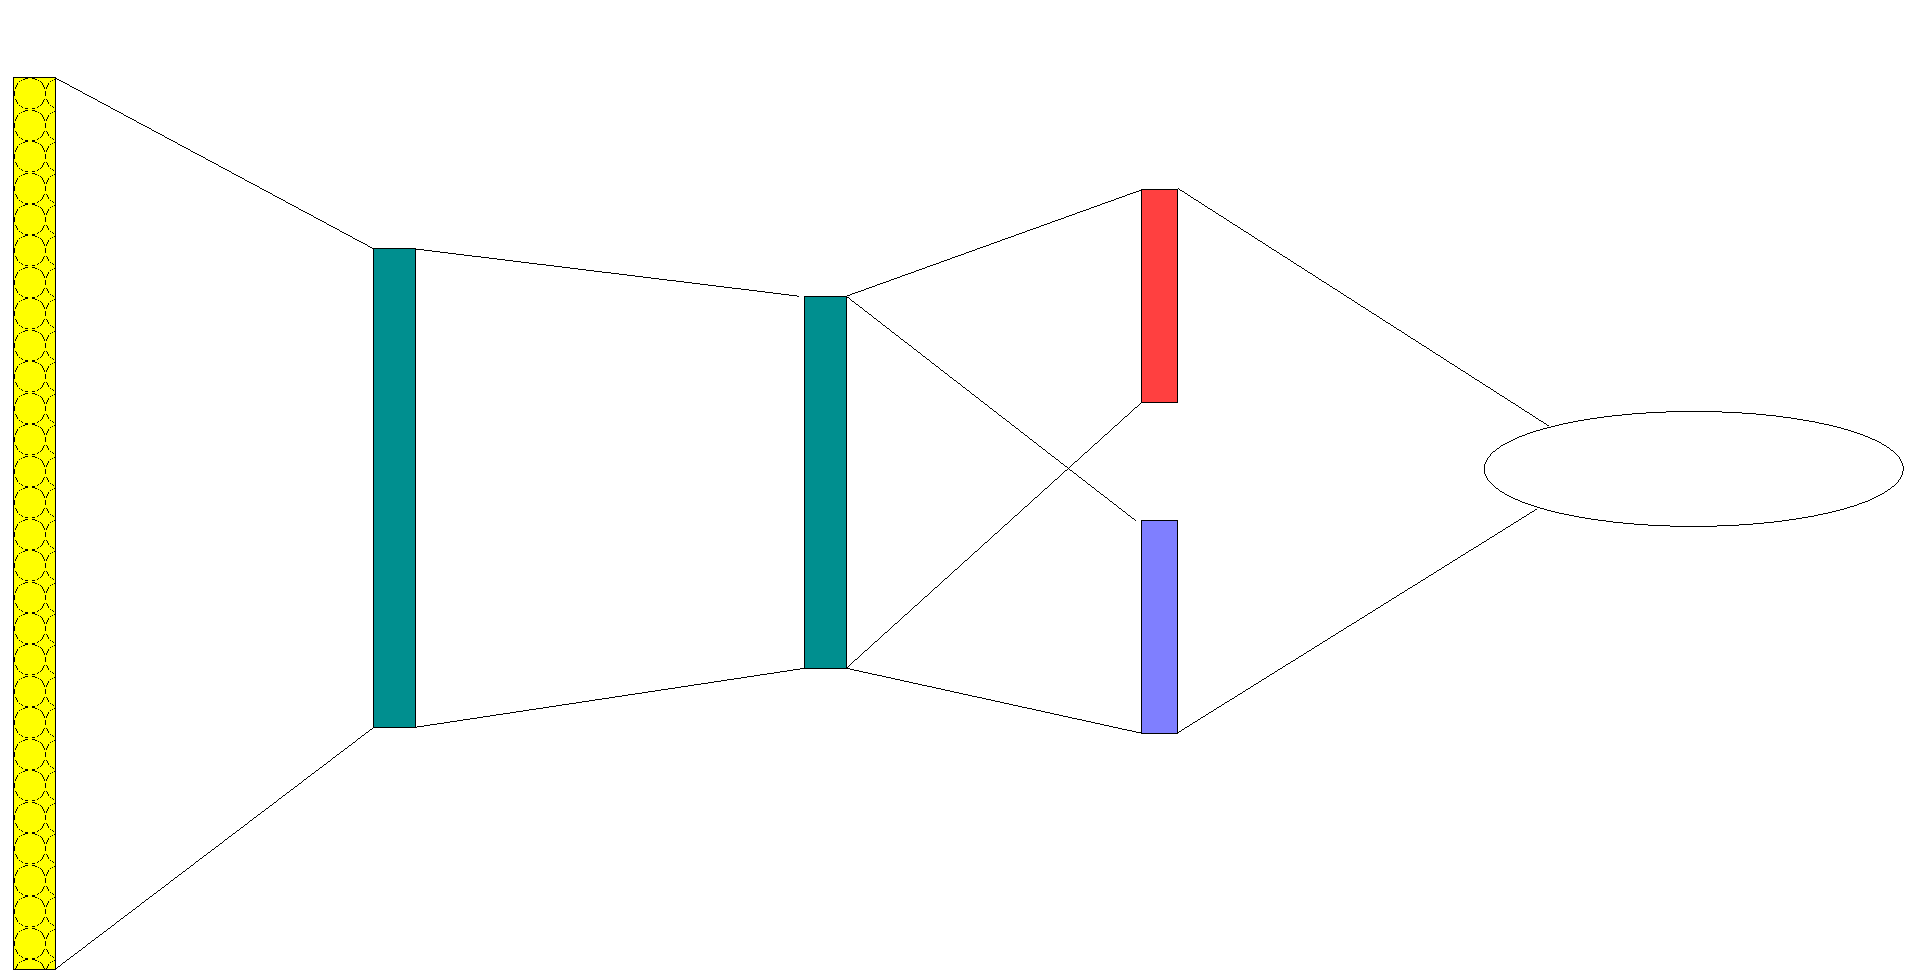
\includegraphics{figures/archi.pdf}%
\end{picture}%
\setlength{\unitlength}{4144sp}%
%
\begingroup\makeatletter\ifx\SetFigFont\undefined%
\gdef\SetFigFont#1#2#3#4#5{%
  \reset@font\fontsize{#1}{#2pt}%
  \fontfamily{#3}\fontseries{#4}\fontshape{#5}%
  \selectfont}%
\fi\endgroup%
\begin{picture}(14512,7383)(3361,-7948)
\put(6121,-2131){\makebox(0,0)[lb]{\smash{{\SetFigFont{29}{34.8}{\rmdefault}{\mddefault}{\updefault}$n_1^h$}}}}
\put(3376,-916){\makebox(0,0)[lb]{\smash{{\SetFigFont{29}{34.8}{\rmdefault}{\mddefault}{\updefault}$n^v$}}}}
\put(7066,-6676){\makebox(0,0)[lb]{\smash{{\SetFigFont{20}{24.0}{\rmdefault}{\mddefault}{\updefault}hidden layers}}}}
\put(10441,-5236){\makebox(0,0)[lb]{\smash{{\SetFigFont{20}{24.0}{\rmdefault}{\mddefault}{\updefault}soft max}}}}
\put(10036,-3076){\makebox(0,0)[lb]{\smash{{\SetFigFont{20}{24.0}{\rmdefault}{\mddefault}{\updefault}fully connected}}}}
\put(7021,-4246){\makebox(0,0)[lb]{\smash{{\SetFigFont{20}{24.0}{\rmdefault}{\mddefault}{\updefault}fully connected}}}}
\put(11926,-1321){\makebox(0,0)[lb]{\smash{{\SetFigFont{29}{34.8}{\rmdefault}{\mddefault}{\updefault}$2n$}}}}
\put(9406,-2131){\makebox(0,0)[lb]{\smash{{\SetFigFont{29}{34.8}{\rmdefault}{\mddefault}{\updefault}$n_2^h$}}}}
\put(3421,-4471){\makebox(0,0)[lb]{\smash{{\SetFigFont{50}{60.0}{\rmdefault}{\mddefault}{\updefault}$X$}}}}
\put(15166,-4246){\makebox(0,0)[lb]{\smash{{\SetFigFont{29}{34.8}{\rmdefault}{\mddefault}{\updefault}$(\hat y(x),\hat I(x))$}}}}
\put(12061,-2941){\makebox(0,0)[lb]{\smash{{\SetFigFont{50}{60.0}{\rmdefault}{\mddefault}{\updefault}$\hat {\bf y}$}}}}
\put(12061,-5506){\makebox(0,0)[lb]{\smash{{\SetFigFont{50}{60.0}{\rmdefault}{\mddefault}{\updefault}$\hat {\bf p}$}}}}
\end{picture}%
}}
\caption{\label{fig:archi} Architecture of the neural network specified by the number of units 
$(n^v,n_1^h,n_2^h,2\vert T\vert)$ in each layer.}
\label{fig:NN}
\end{figure}

\section{Experimental Setting}\label{sec:exp}

%Proofs of concept for the  \XX\ algorithm are obtained using synthetic problems as well as our real-world %motivating application, the prediction of the solar wind (section \ref{sec:intro}). 
The goal of the experiments is twofold. Firstly, the \XX\ predictive performance is assessed by considering i) the MSE of the predicted effect series $\hat y_m$, computed from Eq. (\ref{prop:opred}); 
ii) the accuracy of the timelag prediction. The latter performance indicator is measured and compared to the ground truth using synthetic problems, detailed below: although time lag relationships do exist in real world data sets \citep{doi:10.1002/jgra.50429,ZHOU2006195}, we are not aware of datasets with time lag relationships explicitly annotated. The former performance indicator is comparatively assessed using the naive baseline, the regression model computed by assuming a fixed timelag set to $\frac{\tau_{min}+\tau_{max}}{2}$. The Pearson correlation of the true $y_m$ and predicted $\hat y_m$ series is also considered as overall performance indicator of the prediction.\\
The second goal of experiments is to determine how informative are the key statistical quantities $\sigma_0$ and $C_1$ (section \ref{sec:stability}), and whether they can effectively be used as measures of confidence about the prediction results. 

%said at the end
%The dimensions of the synthetic and real problems used for validation are summarized in Table \ref{tab:exp}.

\paragraph{In synthetic problems,} the driving force $x_m$ of the artificial system is generated in $\mathbb{R}^{10}$ using \emph{Stochastic Langevin Dynamics} (with $\eta = 0.02, s^2 = 0.7$); the time series $y_m$ is generated using the norm of $x_m$: 
\begin{align}
 x_{m+1} &= (1 - \eta) x_m + \mathcal{N}(0, s^2) \label{eq:data}\\
 y_{m+\tau(x_m)} &= k ||x_m||^2 + c \label{eq:outputs}
\end{align}
Four models of increasing complexity have been used for the time lag relationship $\tau(x_m)$; the width of the time lag interval $|T|$ is set to 20 except for Problem I where it is set to 15.\\

{\bf Problem I}: Constant timelag $\tau(x_m) = 5$

In all other problems, the timelag $\tau(x_m)$ depends on the system velocity $v_m = k ||x_m||^2 + c$: 

{\bf Problem II}: Constant velocity $\tau(x_m) = 100/v_m,\ k = 1,\ c = 10$

{\bf Problem III}: Constant acceleration $\tau(x_m) = (\sqrt{v_m^2 + 2ad} - v)/a,\ k = 5,\ a = 5,\ d = 1000, \ c = 100$

{\bf Problem IV}: Softplus $\tau(x_m) = \exp\left(v_m\right)/\left(1 + \exp(v_m/20)\right), \ k = 10, c = 40$

\paragraph{Solar Wind Speed Prediction}\label{sec:solarwind}
As said in section \ref{sec:intro}, the task of predicting solar wind speed from heliospheric data not only 
has huge economic impacts; it is also challenging due to the distance between the Sun and the Earth and the non-stationary propagation time of the solar plasma through the interplanetary medium. 

The $x_m$ series is the solar magnetic \emph{flux tube expansion} (FTE) data produced by the {current sheet source surface} \citep{csss} model, exploiting the hourly magnetogram data recorded by the \emph{Global Oscillation Network Group} from 2008 to 2016.
Solar wind data is extracted from the OMNI data base from the \emph{Space Physics Data Facility}\footnote{\url{https://omniweb.gsfc.nasa.gov}.}. The actual time lag ranges between 2 to 5 days. For computational convenience, the data is pre-processed, retaining for $x_m$ and $y_m$ the median value on a six-hour time window. Accordingly, the number $|T|$ of time lag candidates is 12.  
%For each input pattern, time lagged solar wind data is extracted corresponding to minimum and maximum time delays of two and 5 days respectively. Each three day time window is pre-processed by computing sliding six hour medians yielding $|T| = 12$ time slots.

\XX\ is validated using a 4 fold CV, where the test data consists of one (continuous) month from October 2016 to January 2016. The performance is assessed comparatively to the best state of the art method \citep{Poduval_2014,neuralnetsw}, using  the FTE data and assuming a constant propagation time when combining FTE data with solar wind speed measurements close to the Earth. 

Table \ref{tab:exp} summarizes the dimensions of the synthetic and real problems used as proofs of concept for the \XX\ validation.
\begin{table}[htbp]
  \caption{Synthetic and Real-World Problems}\label{tab:exp_data_info}
  \centering
  \begin{tabular}{ r c c c c}
  \hline
  Problem &  \# train & \# test & $d$ & $|T|$ \\
  \hline
  \textbf{I} & $10,000$ & $2,000$  & $10$ & $15$\\
  \textbf{II} & $10,000$ & $2,000$ & $10$ & $20$\\
  \textbf{III} & $10,000$ & $2,000$ & $10$ & $20$\\
  \textbf{IV} & $10,000$ & $2,000$ & $10$ & $20$\\
  \textbf{Solar Wind} & $77,367$ & $2,205$ & $180$ & $12$\\
  \hline
  \end{tabular}
  \label{tab:exp}
\end{table}

\section{Empirical validation}\label{sec:proofconcept}

\begin{figure*}
  \centering

  \begin{subfigure}[b]{0.4\textwidth}
    \centering
    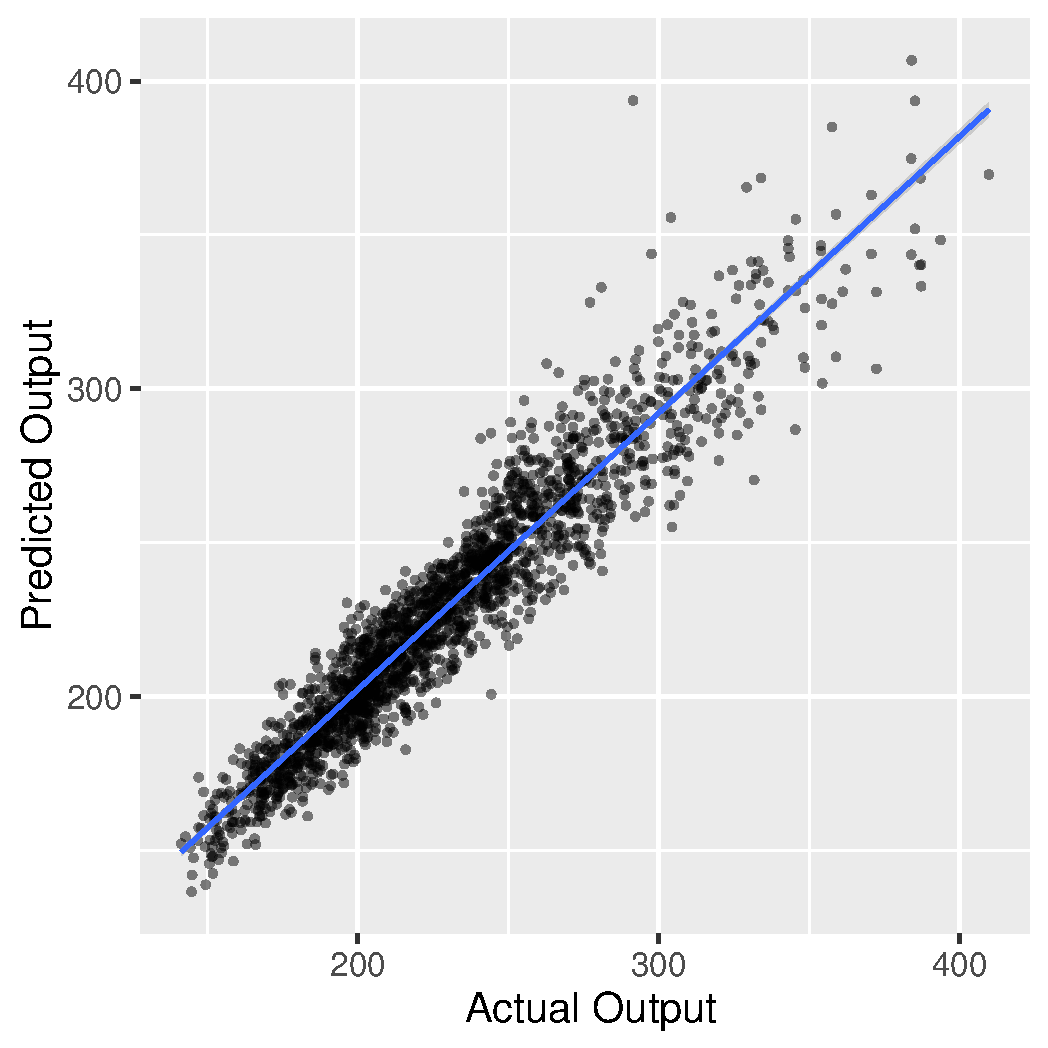
\includegraphics[width=\textwidth]{figures/exp2_scatter_v_test}
    \caption{ \textbf{Problem II}, Goodness of fit, Output $y(x)$}
    \label{fig:problem2_fitv}
  \end{subfigure}
  \hfill
  \begin{subfigure}[b]{0.4\textwidth}
    \centering
    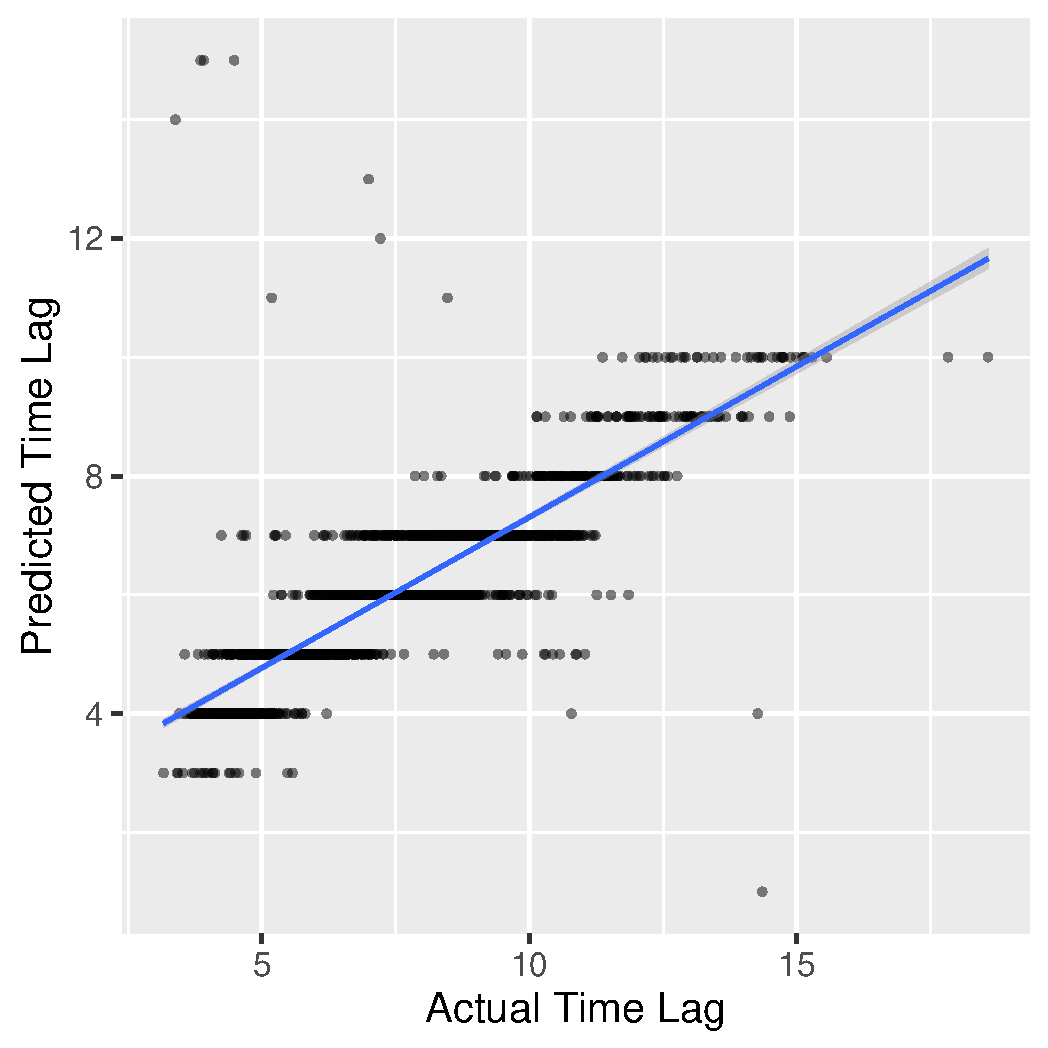
\includegraphics[width=\textwidth]{figures/exp2_scatter_t_test}
    \caption{ \textbf{Problem II}, Goodness of fit, Time lag $\tau(t)$ }
    \label{fig:problem2_fitt}
  \end{subfigure}
  
  \vskip\baselineskip
  
  \begin{subfigure}[b]{0.4\textwidth}
    \centering
    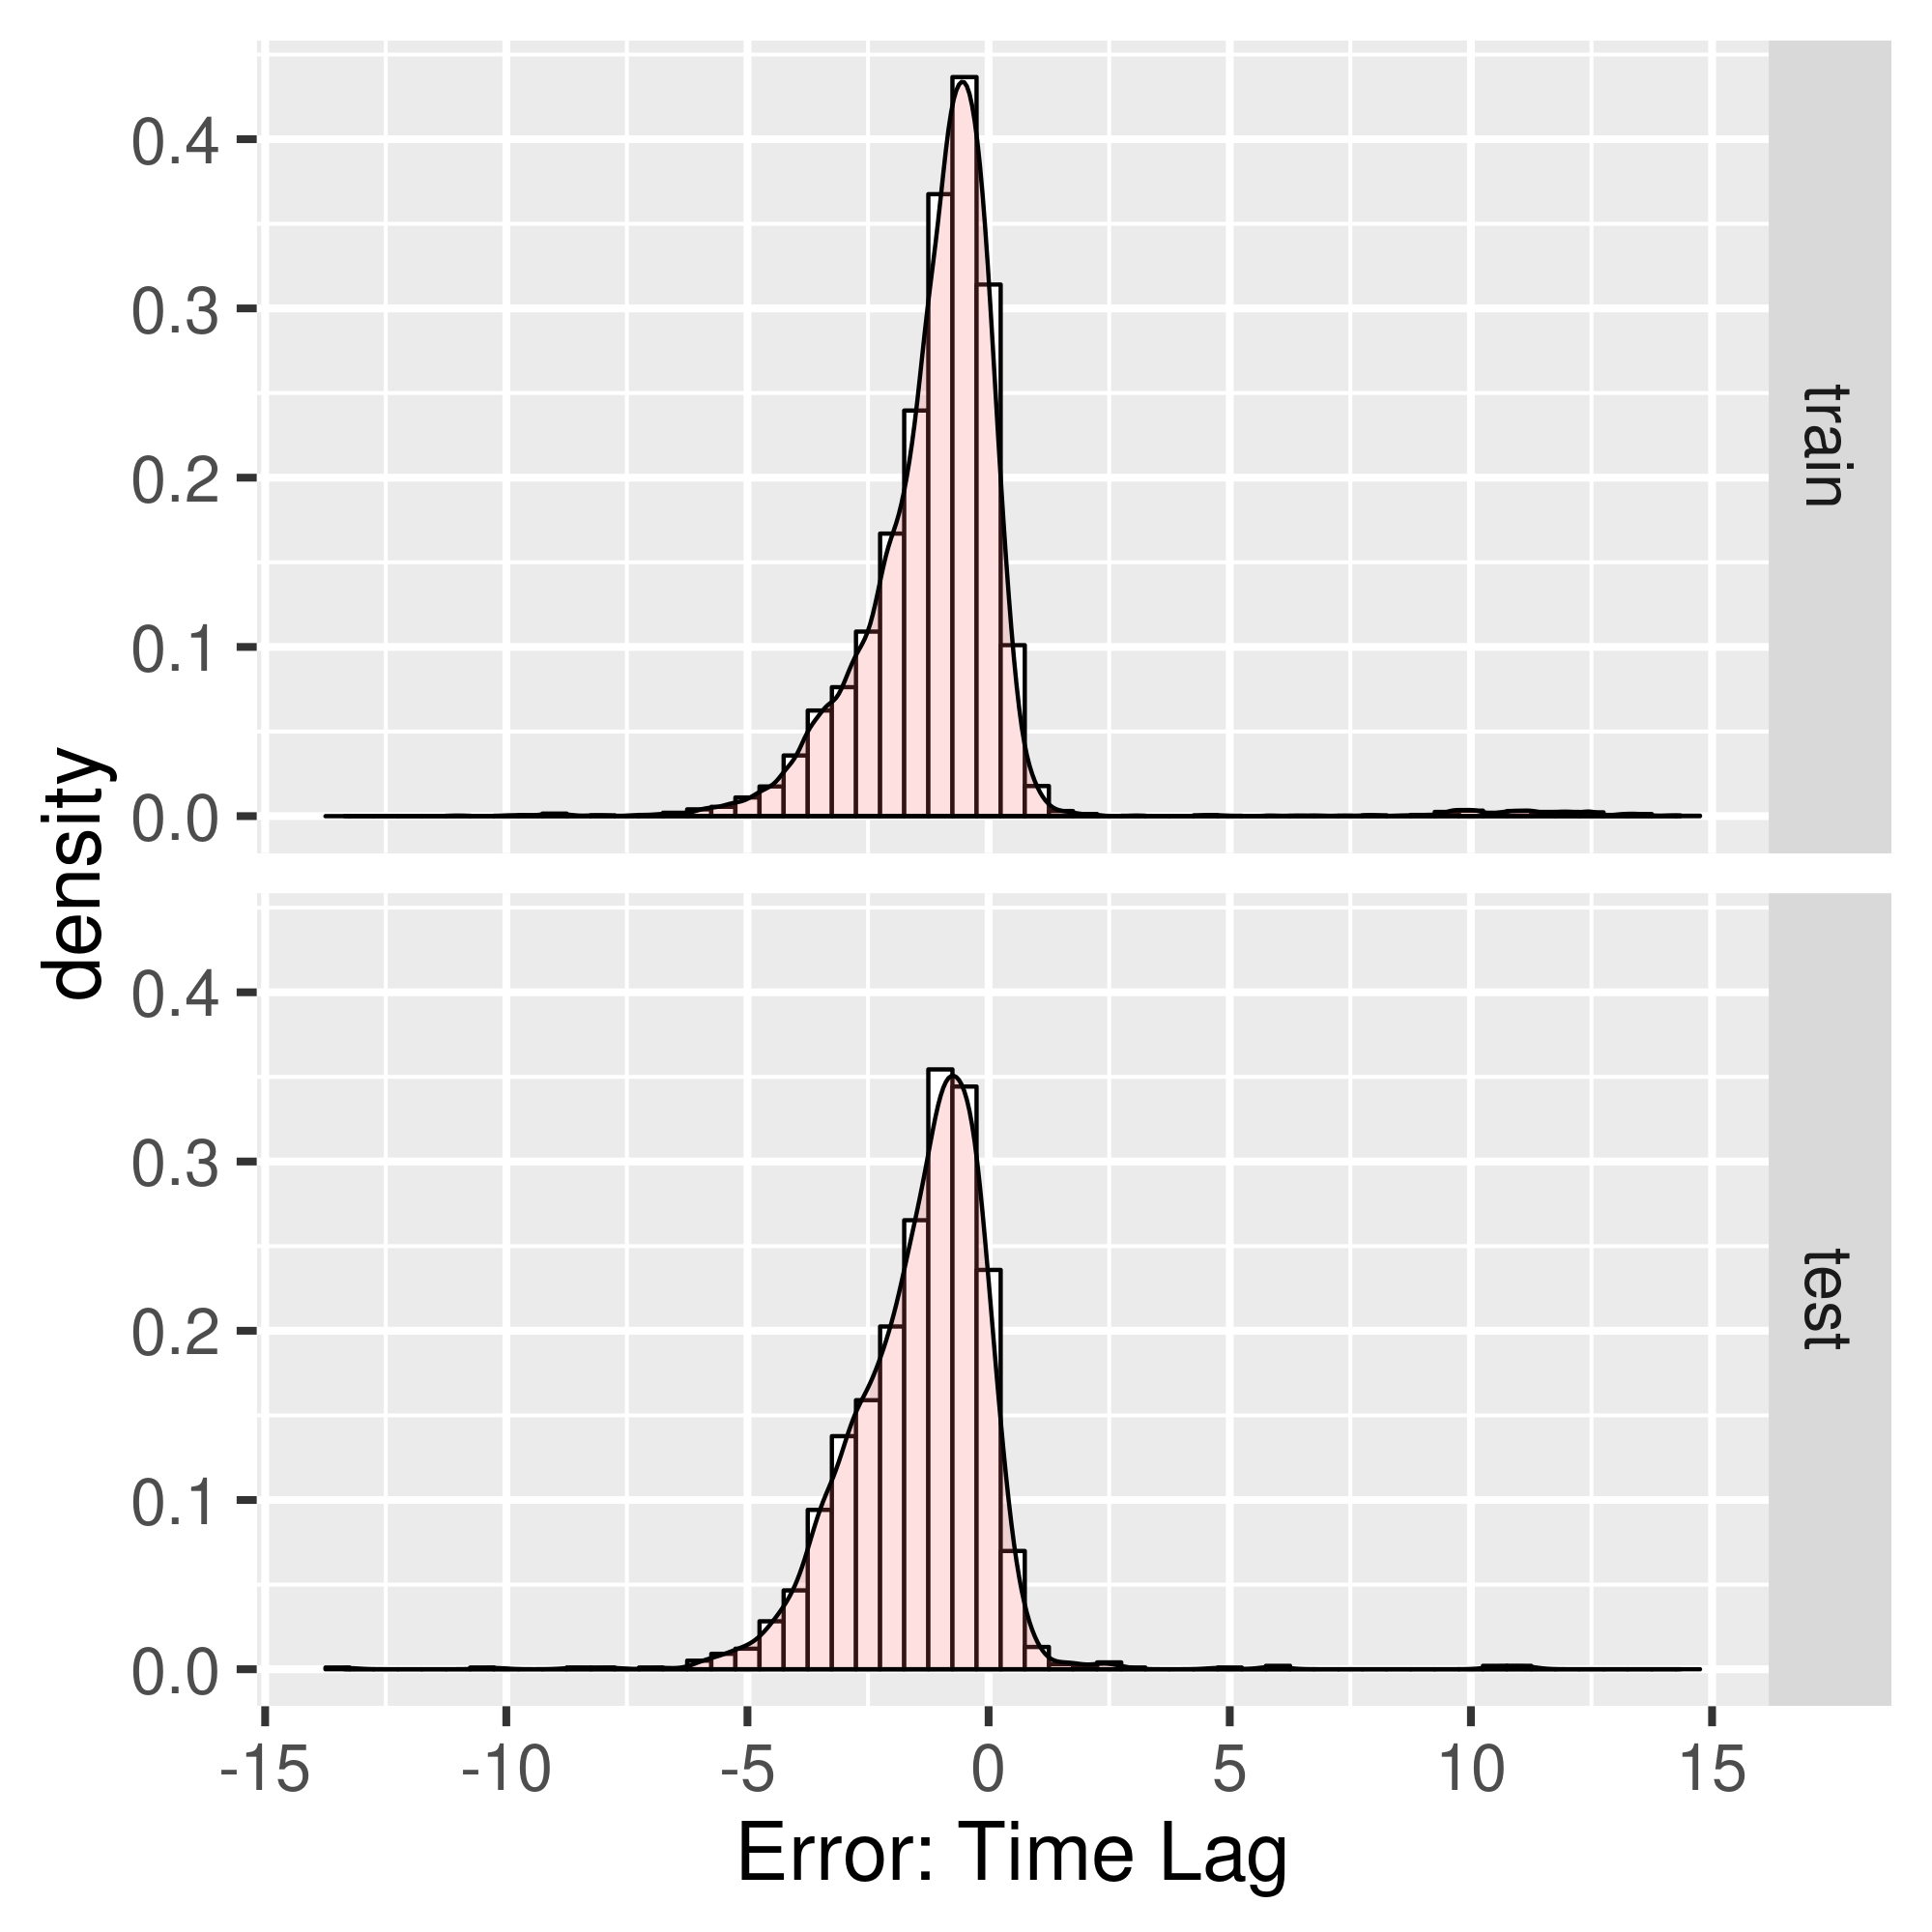
\includegraphics[width=\textwidth]{figures/exp2_hist_errors_timelag}
    \caption{ \textbf{Problem II}, Error of time lag prediction} 
    \label{fig:problem2_error}
  \end{subfigure}
  \hfill
  \begin{subfigure}[b]{0.4\textwidth}
    \centering
    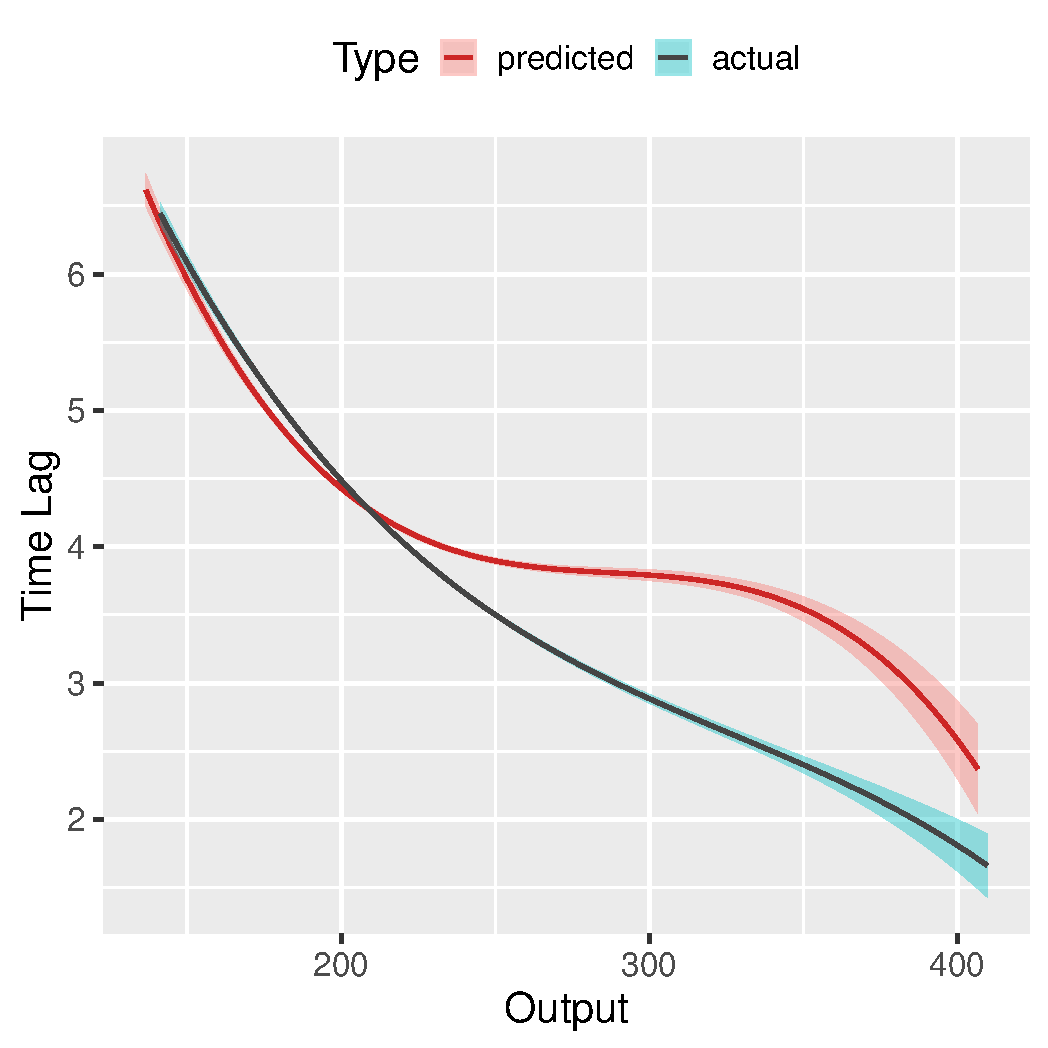
\includegraphics[width=\textwidth]{figures/exp2_predictive_curves}
    \caption{ \textbf{Problem II}, Output vs Time Lag Relationship} 
    \label{fig:problem2_curves}
  \end{subfigure}

  %\vskip\baselineskip
  
  %\begin{subfigure}[b]{0.4\textwidth}
  %  \centering
  %  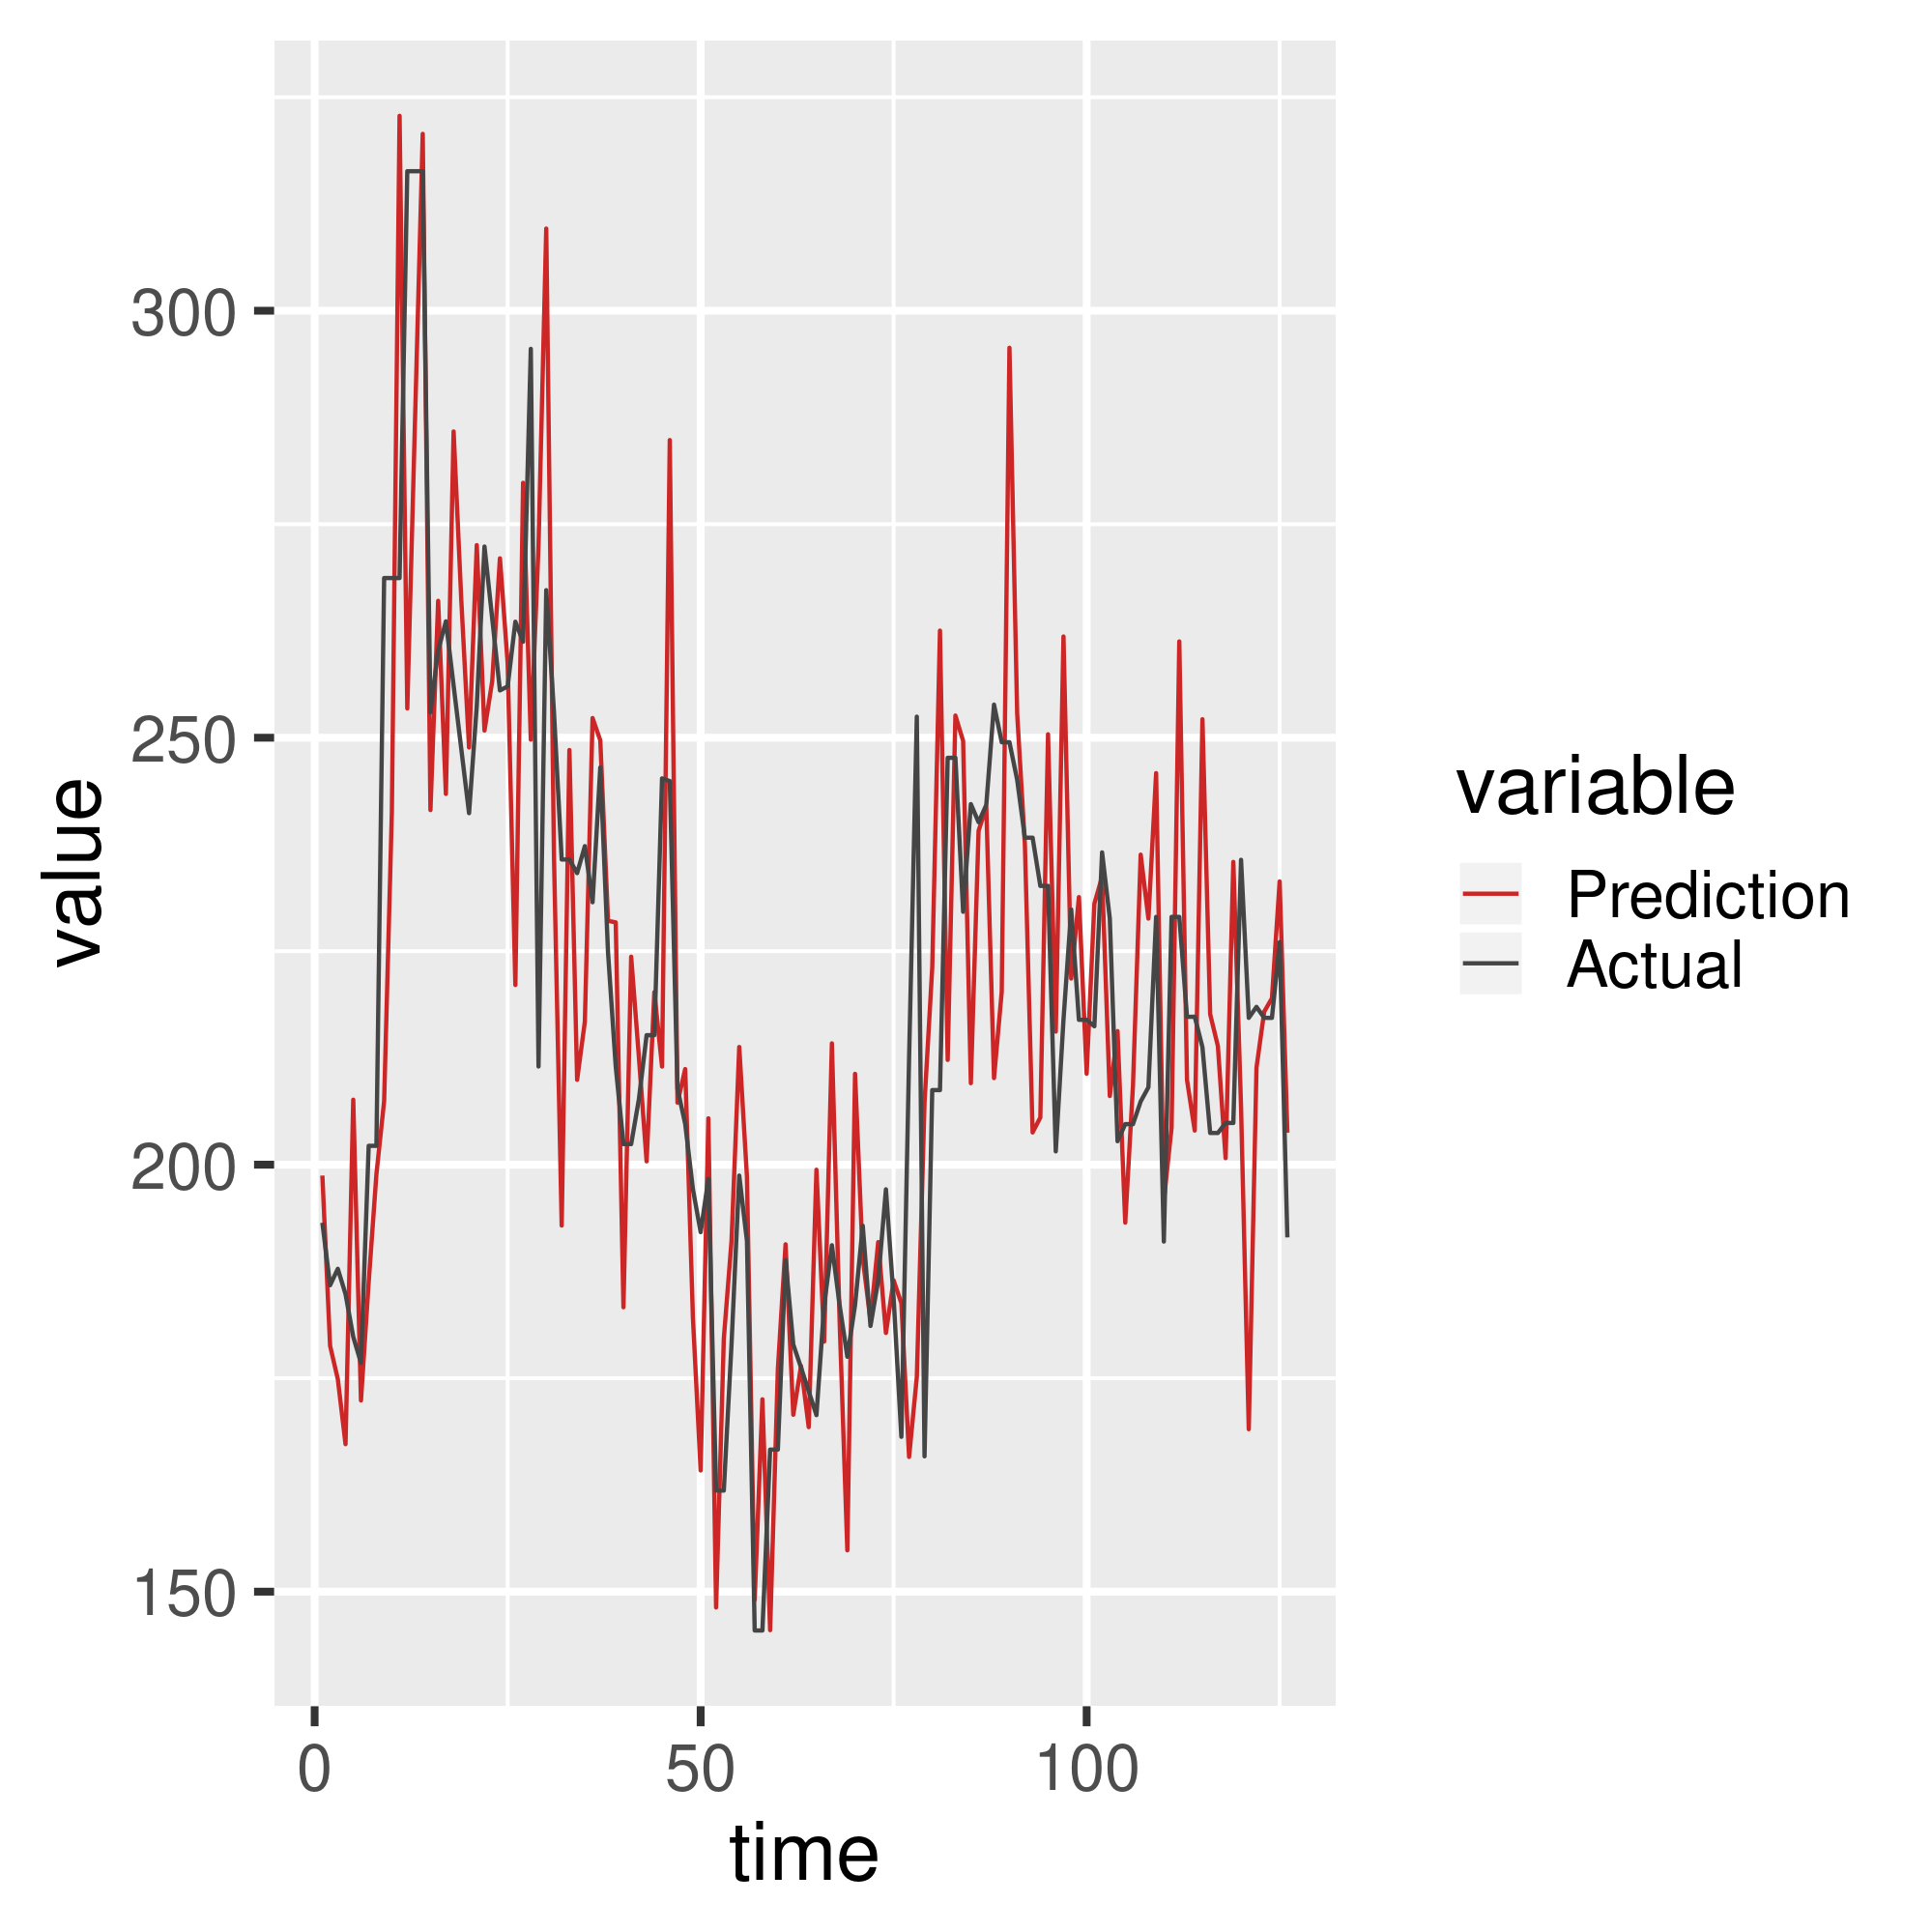
\includegraphics[width=\textwidth]{figures/exp2_timeseries_pred}
  %  \caption{ \textbf{Problem II}, A portion of the test time series reconstructed using the model} 
  %  \label{fig:problem2_timeseries}
  %\end{subfigure}
  %\hfill
  %\begin{subfigure}[b]{0.4\textwidth}
  %  \centering
  %  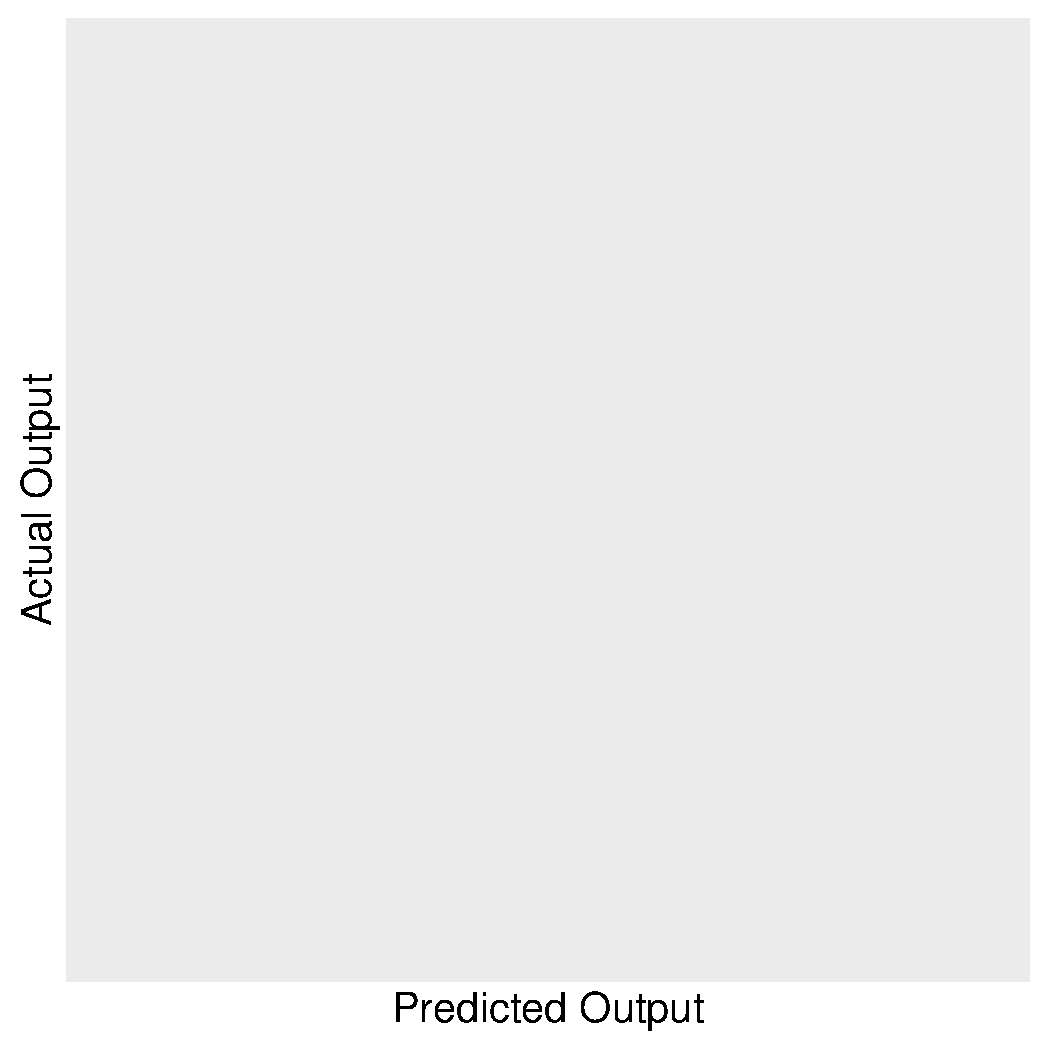
\includegraphics[width=\textwidth]{figures/exp2_lag_error_jus}
  %  \caption{ \textbf{Problem II}, Predicted vs Actual Outputs for the cases with time lag error $\leq -2.5$.} 
  %  \label{fig:problem2_lag_error_jus}
  %\end{subfigure}
  
  \caption{\textbf{Problem II}, Results}
\end{figure*}

\begin{figure*}
  \centering

  \begin{subfigure}[b]{0.4\textwidth}
    \centering
    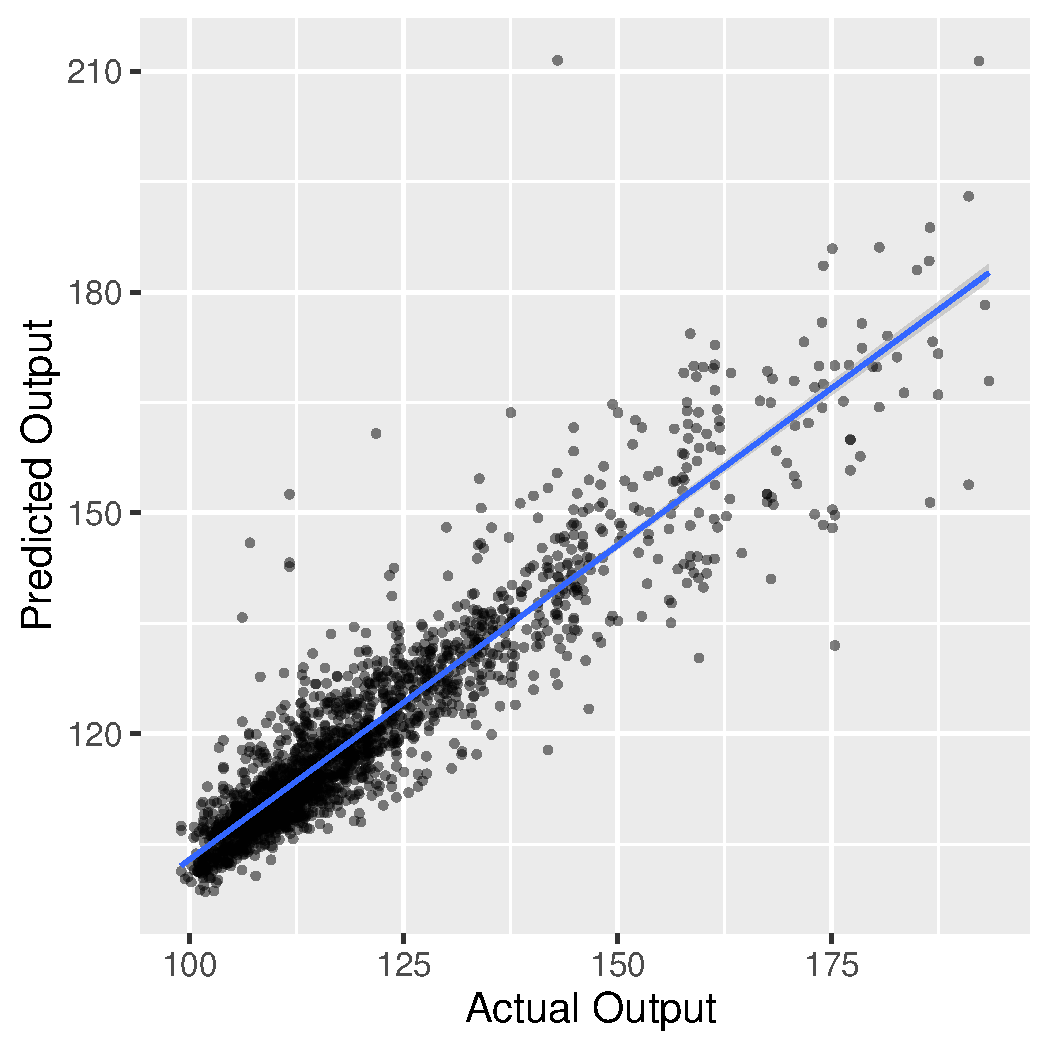
\includegraphics[width=\textwidth]{figures/exp3_scatter_v_test}
    \caption{ \textbf{Problem III}, Goodness of fit, Output $y(x)$}
    \label{fig:problem3_fitv}
  \end{subfigure}
  \hfill
  \begin{subfigure}[b]{0.4\textwidth}
    \centering
    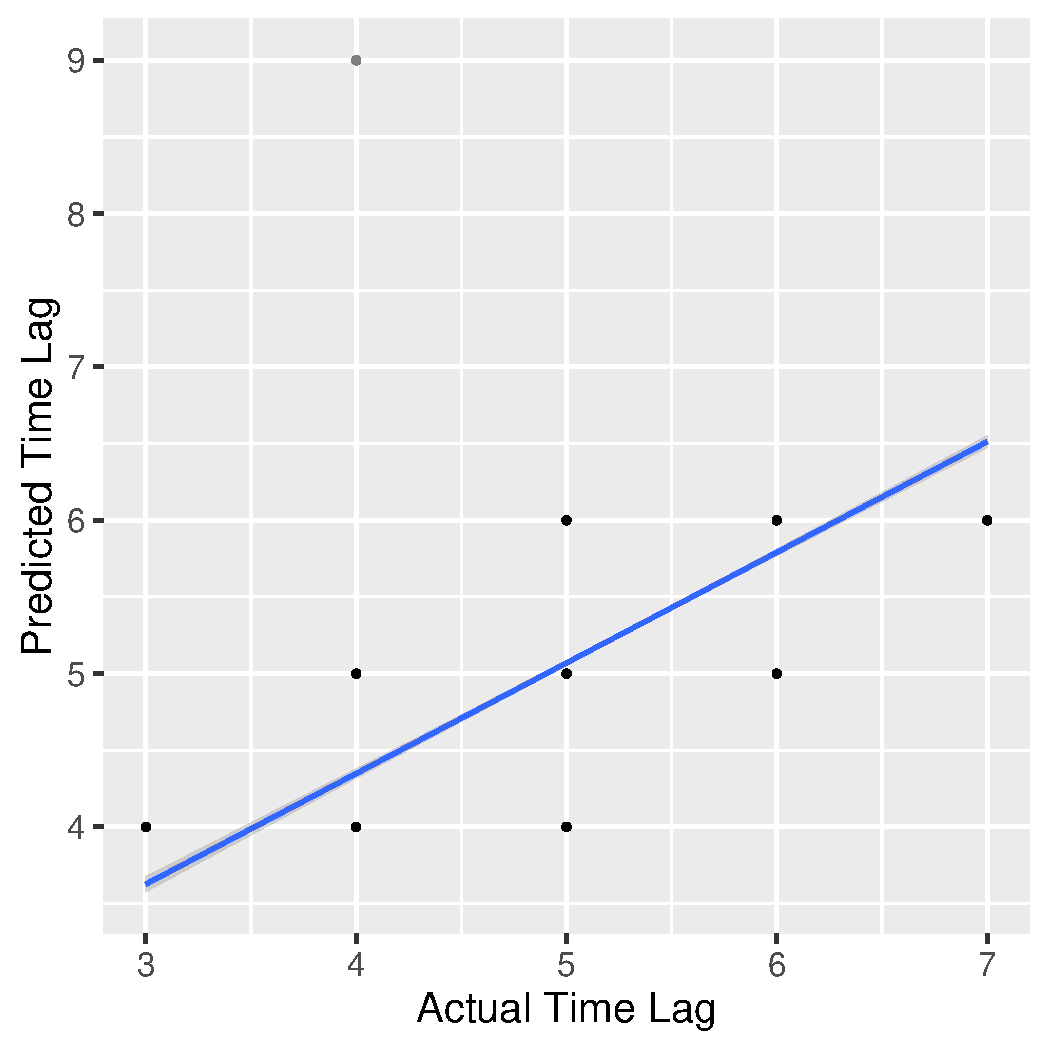
\includegraphics[width=\textwidth]{figures/exp3_scatter_t_test}
    \caption{ \textbf{Problem III}, Goodness of fit, Time lag $\tau(t)$ }
    \label{fig:problem3_fitt}
  \end{subfigure}

  \vskip\baselineskip
  
  \begin{subfigure}[b]{0.4\textwidth}
    \centering
    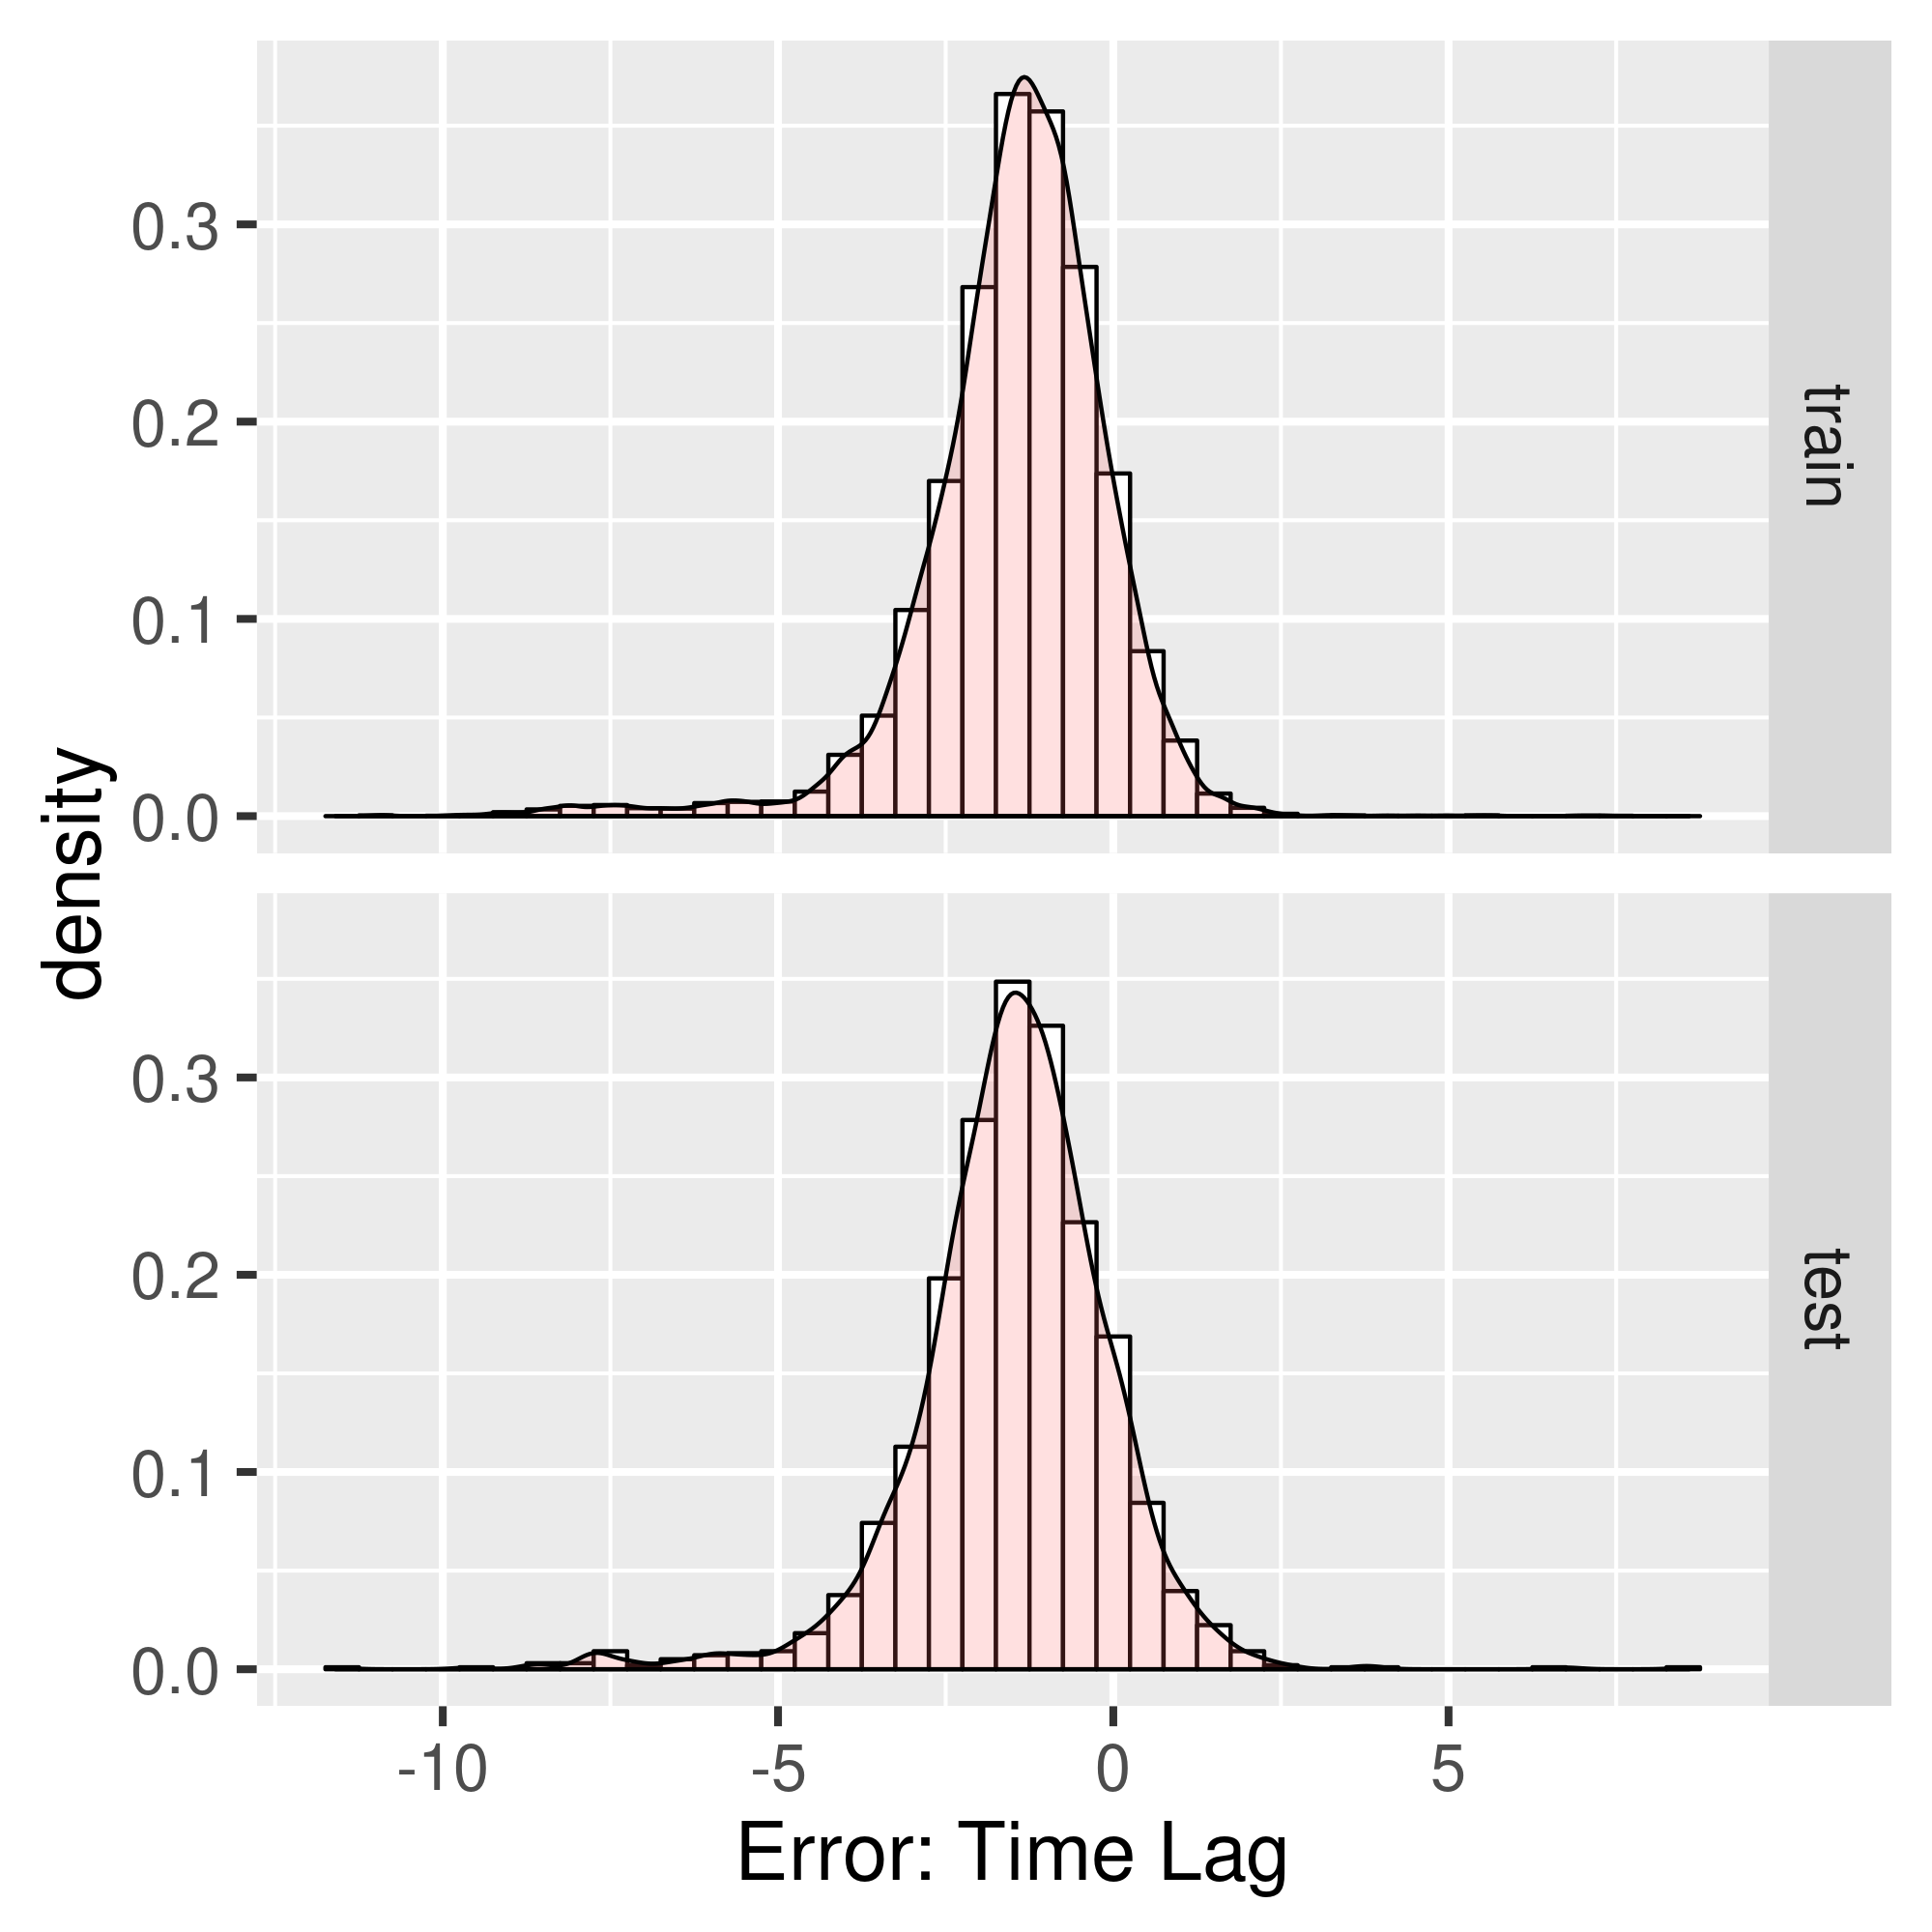
\includegraphics[width=\textwidth]{figures/exp3_hist_errors_timelag}
    \caption{ \textbf{Problem III}, Error of time lag prediction} 
    \label{fig:problem3_error}
  \end{subfigure}
  \hfill
  \begin{subfigure}[b]{0.4\textwidth}
    \centering
    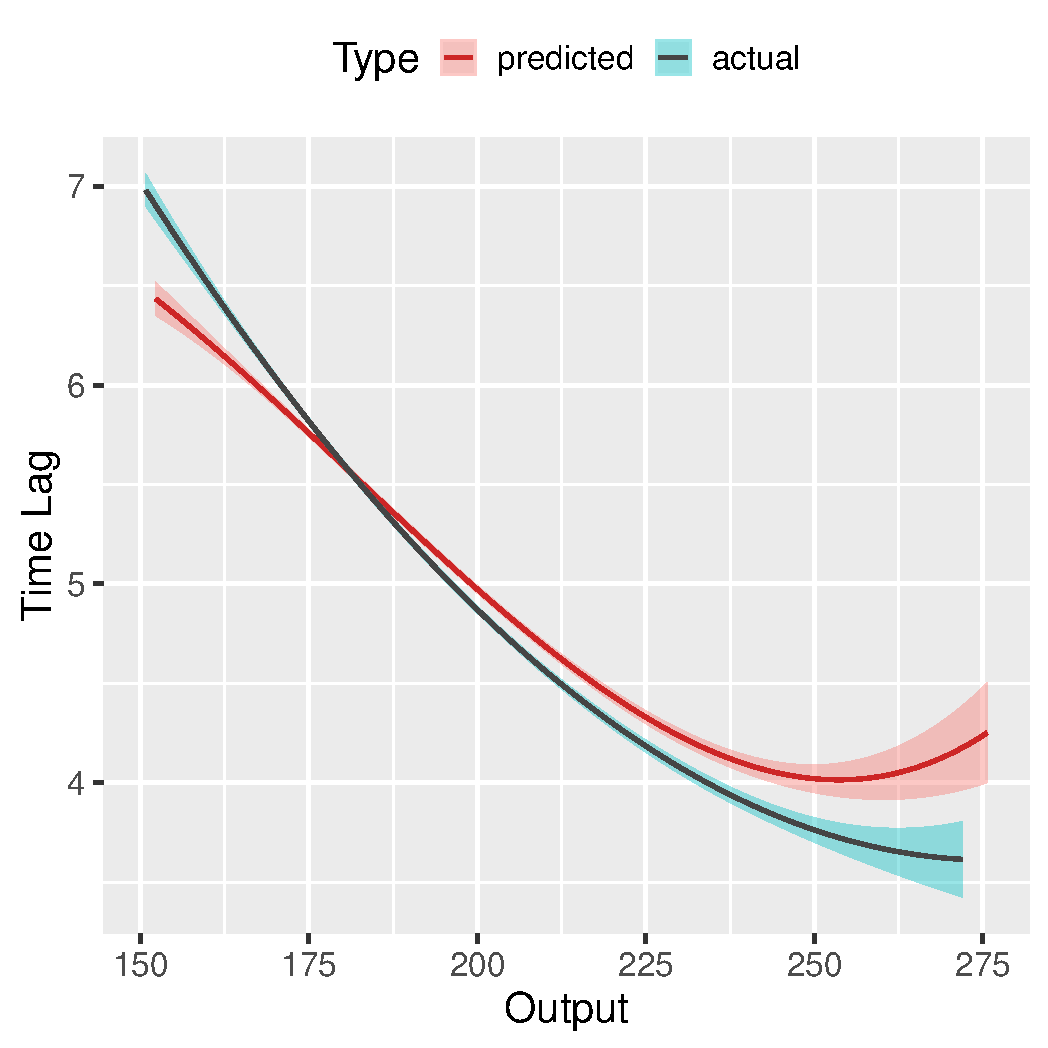
\includegraphics[width=\textwidth]{figures/exp3_predictive_curves}
    \caption{ \textbf{Problem III}, Output vs Time Lag Relationship} 
    \label{fig:problem3_curves}
  \end{subfigure}
  
  %\vskip\baselineskip
  
  %\begin{subfigure}[b]{0.4\textwidth}
  %  \centering
  %  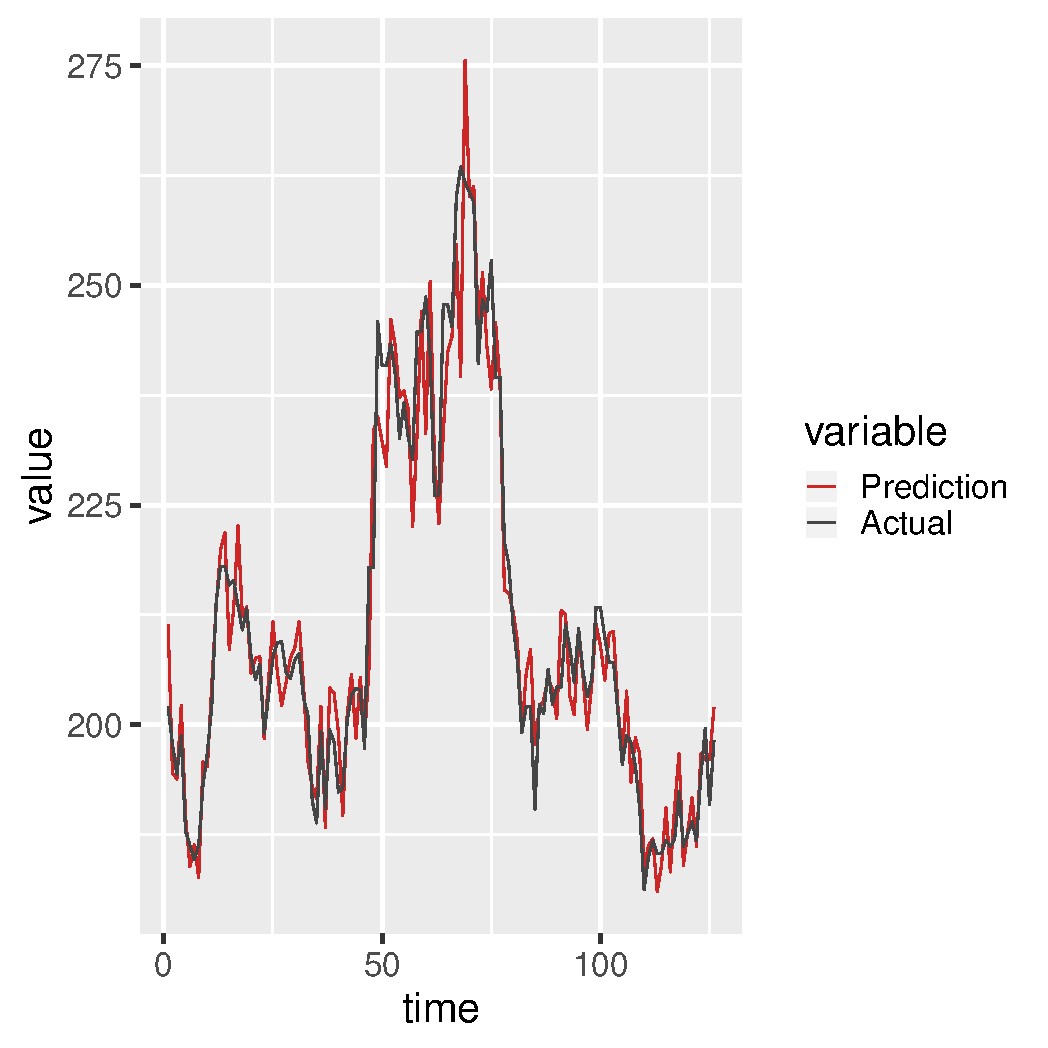
\includegraphics[width=\textwidth]{figures/exp3_timeseries_pred}
  %  \caption{ \textbf{Problem III}, A portion of the test time series reconstructed using the model} 
  %  \label{fig:problem3_timeseries}
  %\end{subfigure}
  %\hfill
  %\begin{subfigure}[b]{0.4\textwidth}
  %  \centering
  %  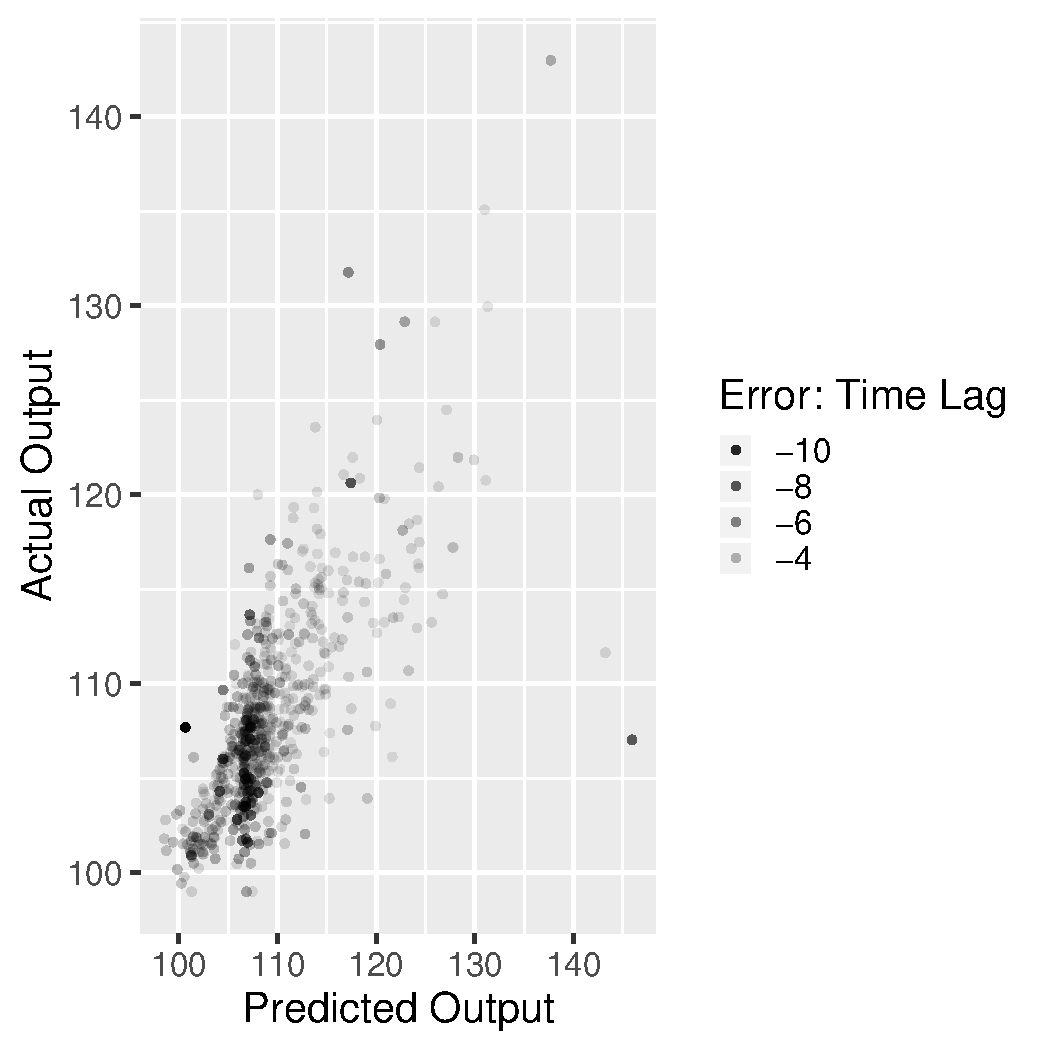
\includegraphics[width=\textwidth]{figures/exp3_lag_error_jus}
  %  \caption{ \textbf{Problem III}, Predicted vs Actual Outputs for the cases with time lag error $\leq -2.5$.} 
  %  \label{fig:problem3_lag_error_jus}
  %\end{subfigure}
  
  \caption{\textbf{Problem III}, Results}
\end{figure*}

\begin{figure*}
  \centering

  \begin{subfigure}[b]{0.4\textwidth}
    \centering
    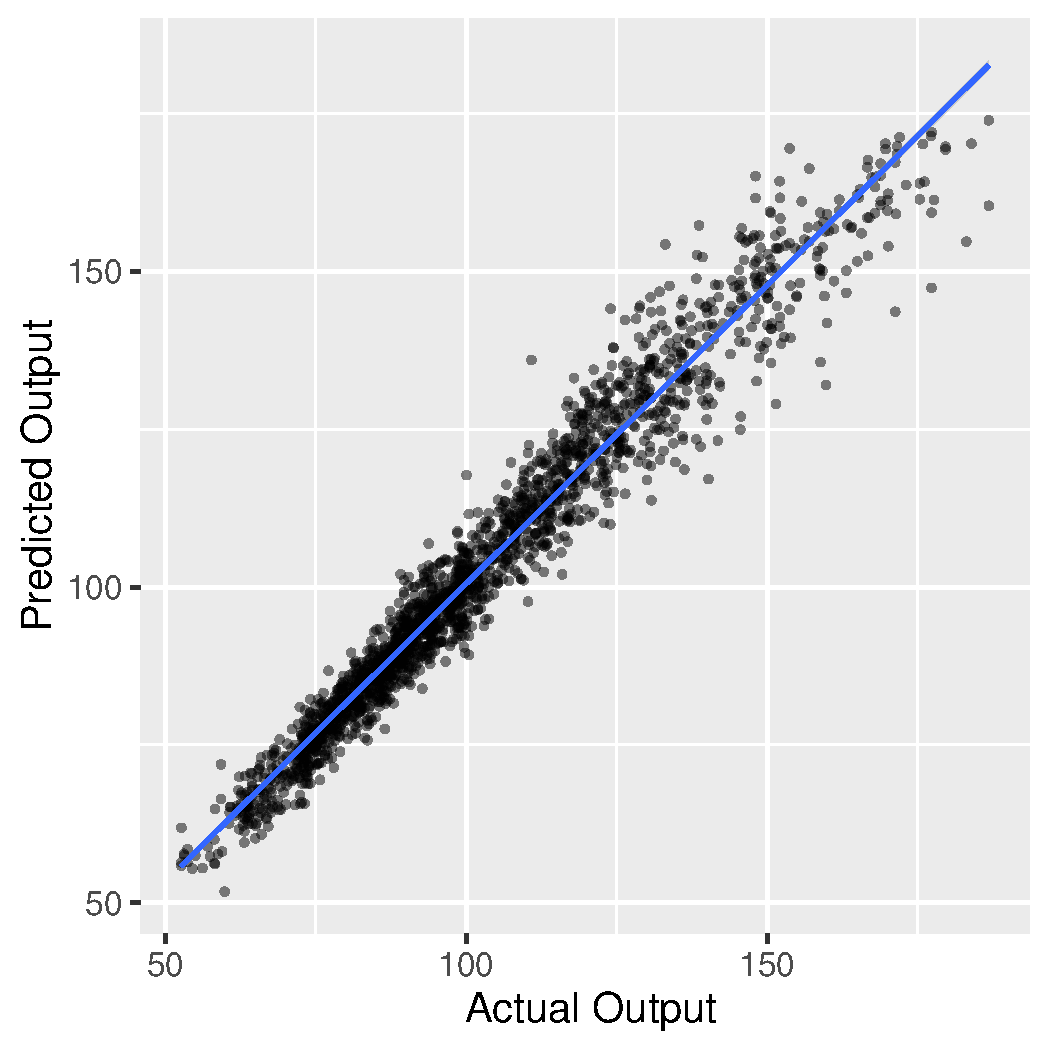
\includegraphics[width=\textwidth]{figures/exp4_scatter_v_test}
    \caption{ \textbf{Problem IV}, Goodness of fit, Output $y(x)$}
    \label{fig:problem4_fitv}
  \end{subfigure}
  \hfill
  \begin{subfigure}[b]{0.4\textwidth}
    \centering
    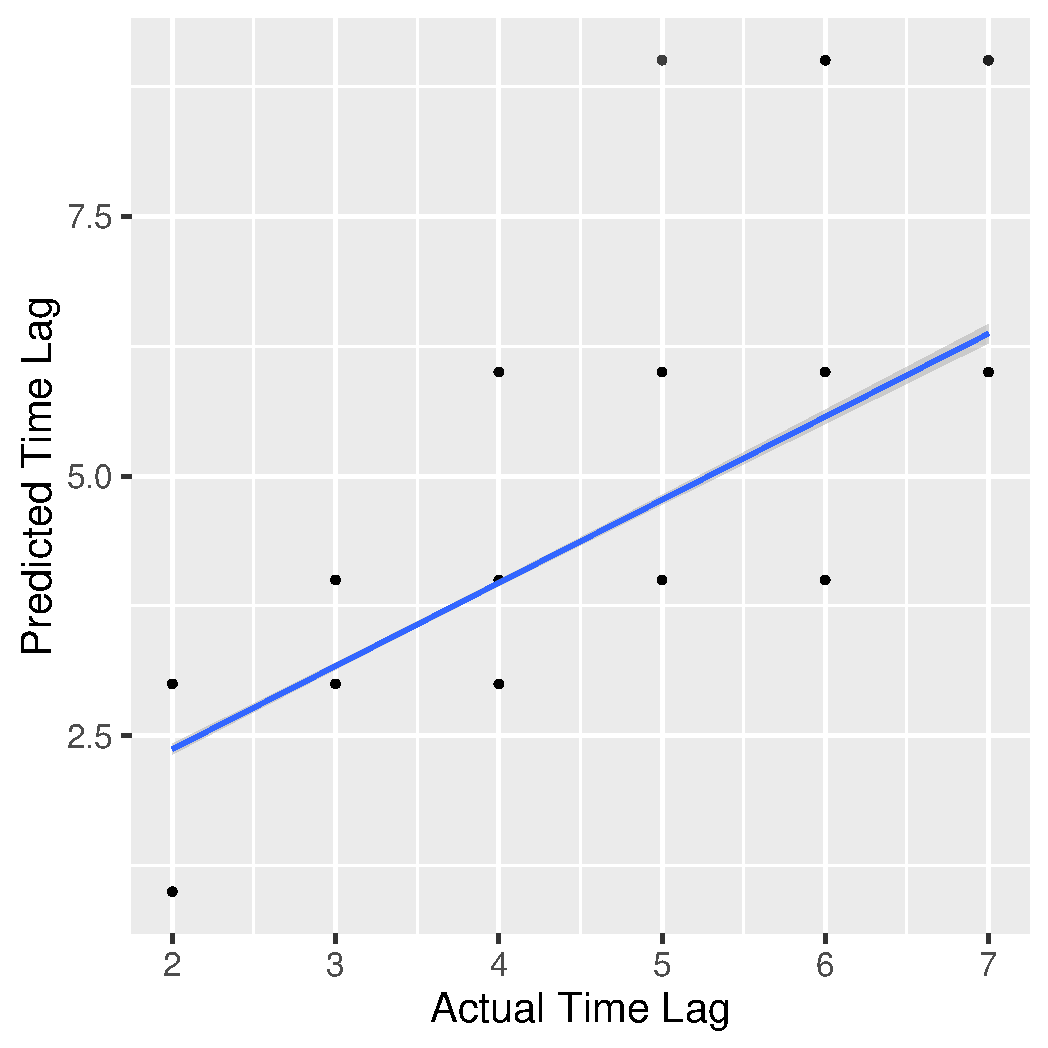
\includegraphics[width=\textwidth]{figures/exp4_scatter_t_test}
    \caption{ \textbf{Problem IV}, Goodness of fit, Time lag $\tau(t)$ }
    \label{fig:problem4_fitt}
  \end{subfigure}
  
  \vskip\baselineskip
  
  \begin{subfigure}[b]{0.4\textwidth}
    \centering
    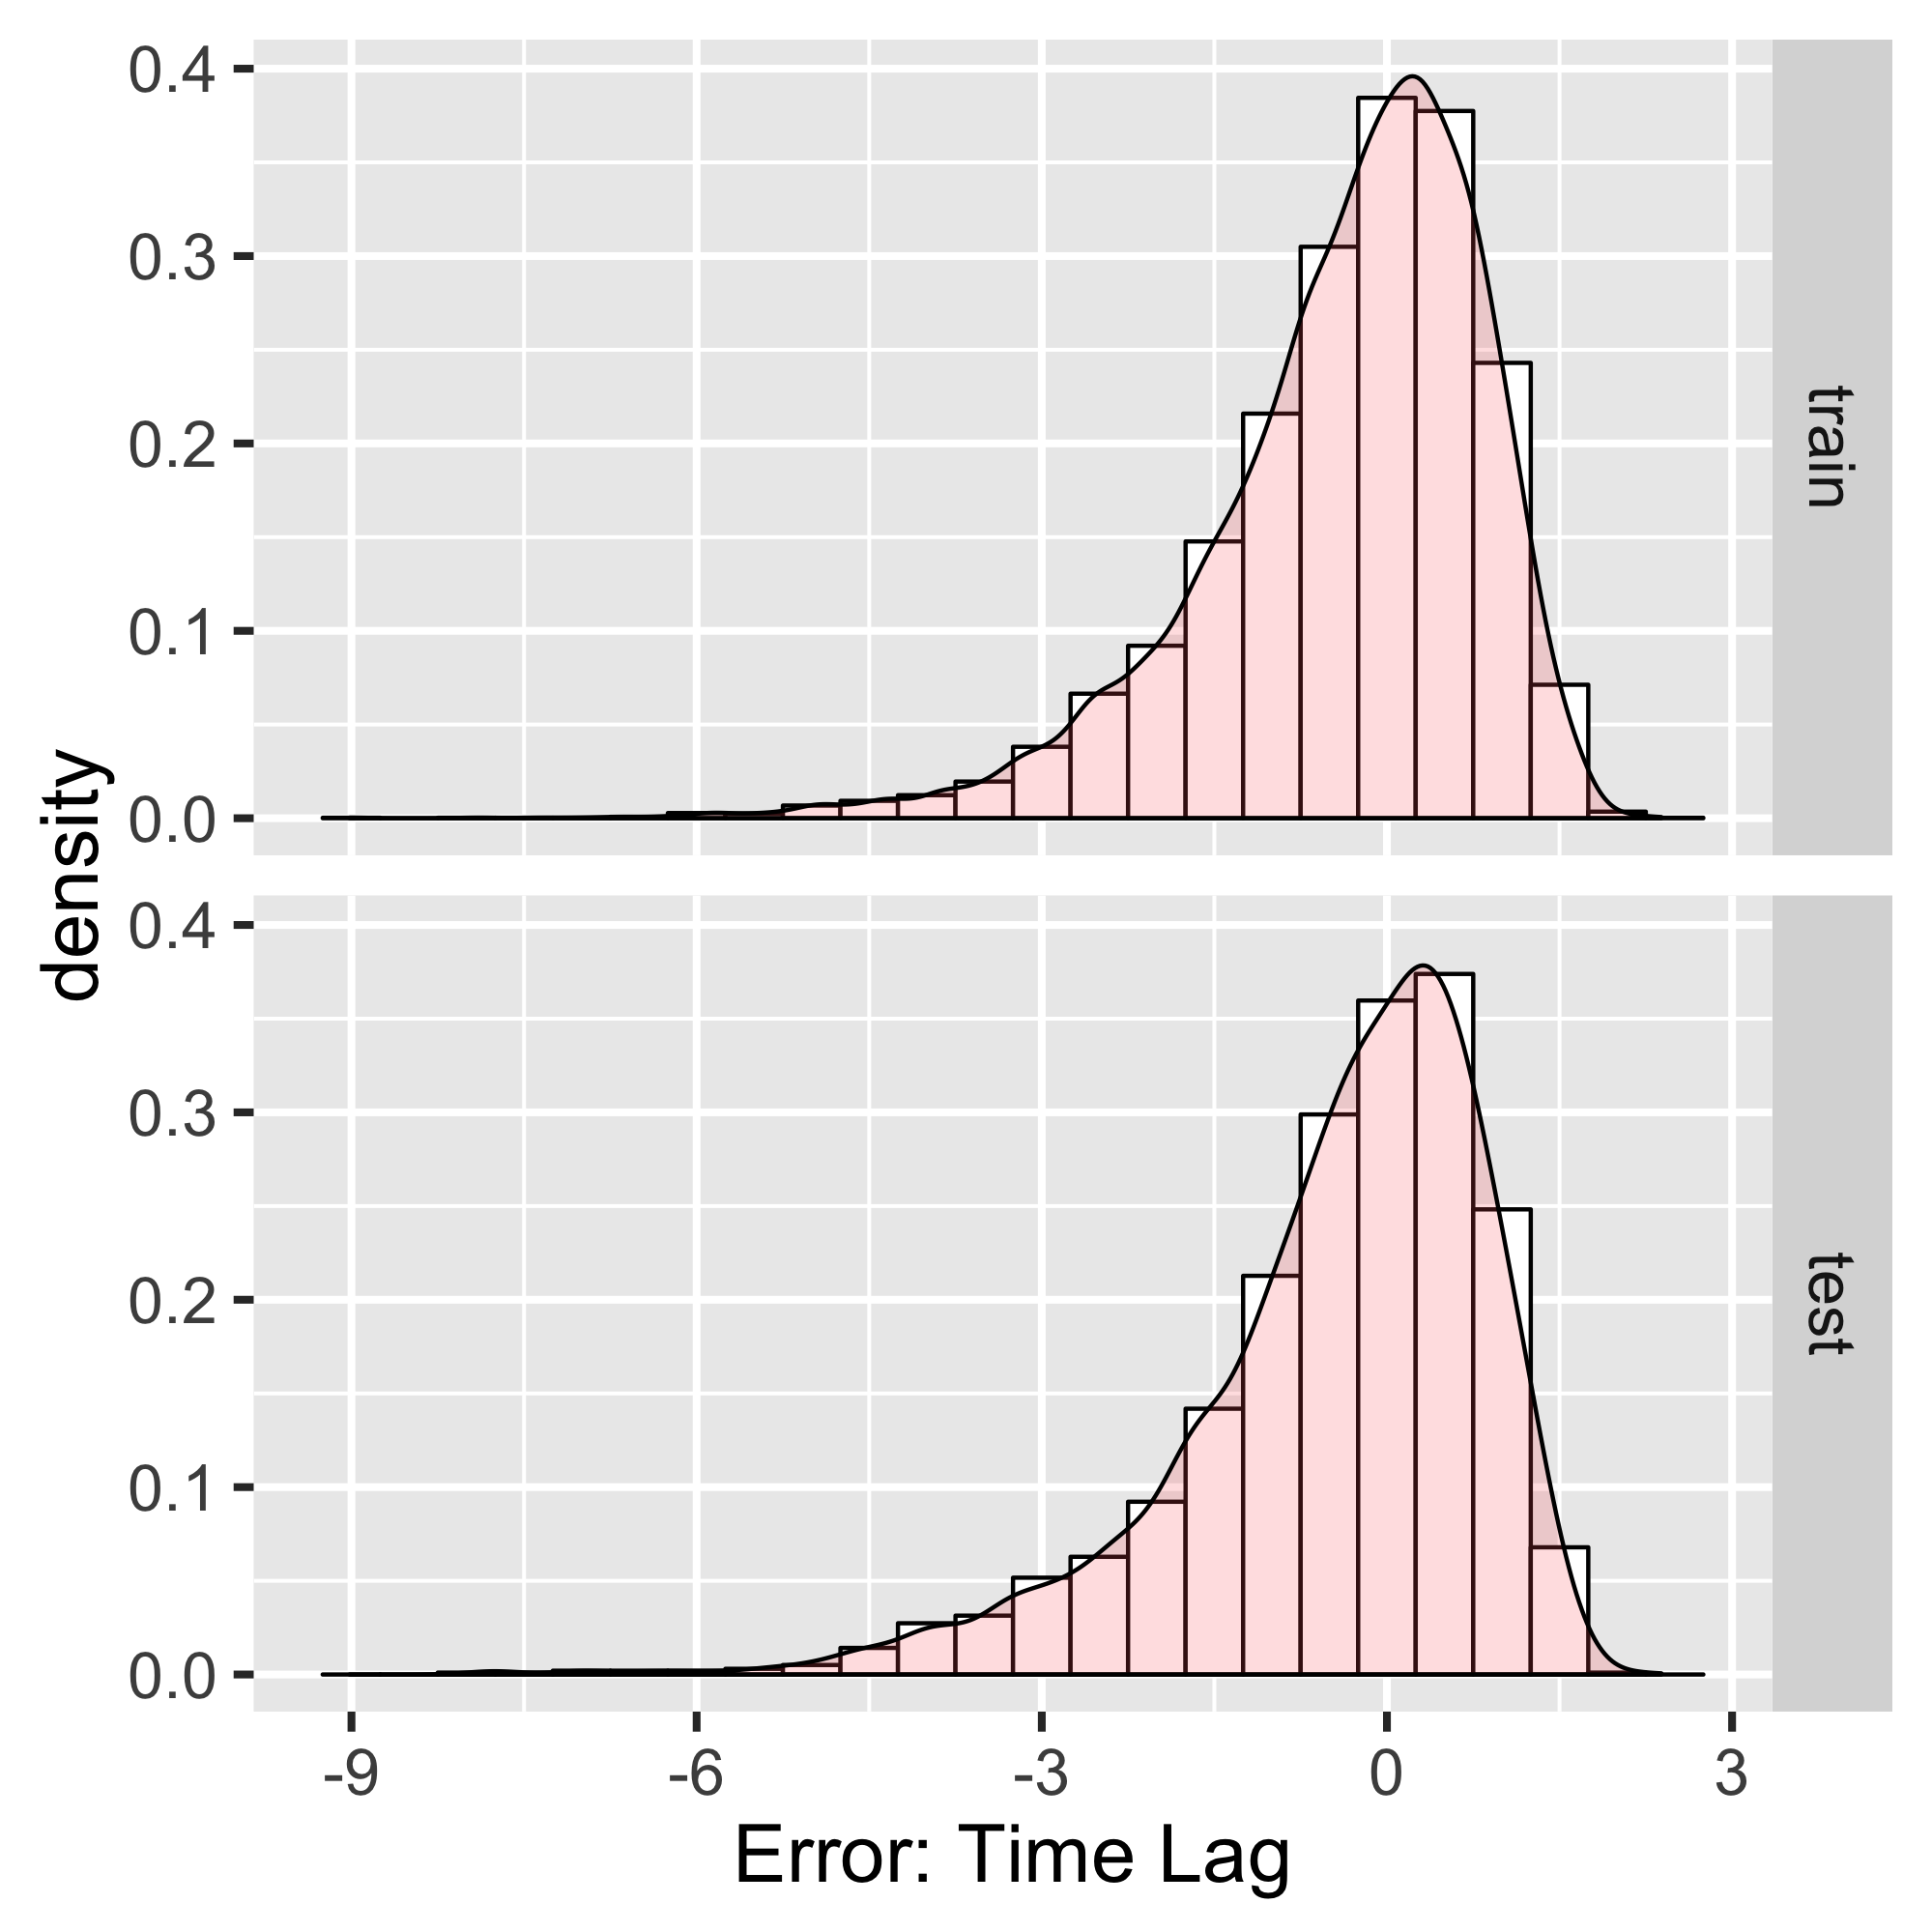
\includegraphics[width=\textwidth]{figures/exp4_hist_errors_timelag}
    \caption{ \textbf{Problem IV}, Error of time lag prediction} 
    \label{fig:problem4_error}
  \end{subfigure}
  \hfill
  \begin{subfigure}[b]{0.4\textwidth}
    \centering
    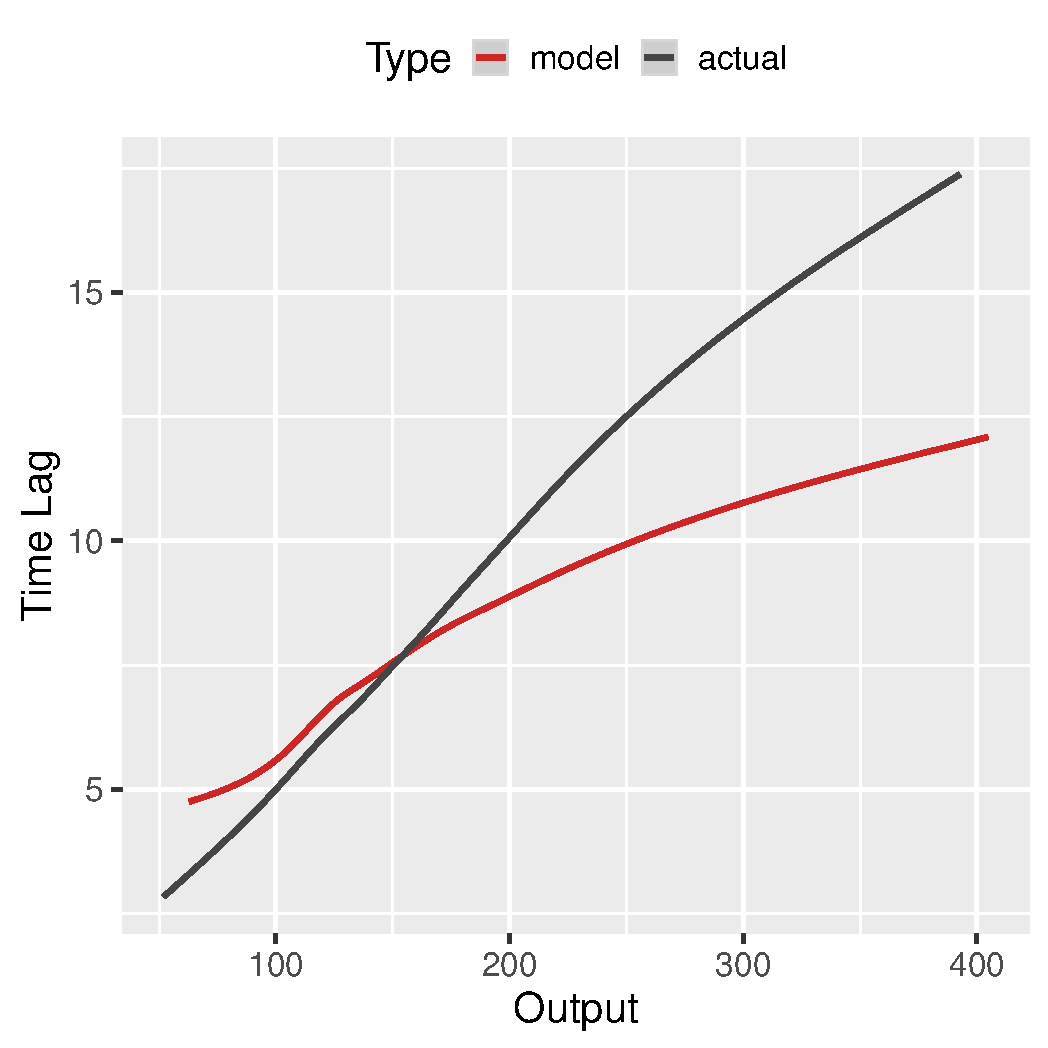
\includegraphics[width=\textwidth]{figures/exp4_predictive_curves}
    \caption{ \textbf{Problem IV}, Output vs Time Lag Relationship} 
    \label{fig:problem4_curves}
  \end{subfigure}
  
  \caption{\textbf{Problem IV}, Results}
\end{figure*}


Table \ref{tab:results_syn} summarizes the \XX\ performance on the synthetic and real-world problems, respectively compared to the naive baseline (constant time lag) and to the state of the art for the real-world solar wind problem (please see supplementary material for more detail, plots of the results and timelag error histogram). 

The values of the $\sigma_0$ and $C_1$ quantities involved in the stability analysis (section \ref{sec:stability}) are also reported. As said, $C_1 < 1$ indicates a specialization among predictors found by the solution. The comparison of $\sigma_0$ and the RMSE indicates how better the learned model is compared to the trivial degenerate solution (uniform $\hat {\bf p}$, assigning an equal weight to all $\hat y_i$). 
Finally, the Pearson correlation between $\hat y_m$ and $y_m$ is reported; while its absolute value is less informative than it appears due to the auto-correlation of the series, it allows to compare different predictors. 

\begin{table}
  \caption{Performance: \XX  \ / Base Line / \XX  \ Time Lag Prediction}\label{tab:results_syn}
  \centering
  \begin{tabular}{ l l l l l l}
  \hline
  Problem &  M.A.E & R.M.S.E & Pearson Corr. & $\sigma_0$ & $C_1$\\
  \hline
  \textbf{Pb I} & $8.82$ / $21.79$ / $0.021$  & $12.35$ / $28.79$ / $0.26$ & $0.98$ / $0.87$ / -- & $29.8$ & $0.14$\\
  \textbf{Pb II} & $10.15$ / $27.40$ / $0.4$ & $13.70$ / $35.11$ / $0.67$ & $0.95$ / $0.73$ / $0.70$ & $26.83$ & $0.16$\\
  \textbf{Pb III} & $3.17$ / $11.01$ / $0.17$ & $4.63$ / $14.99$ / $0.42$ & $0.98$ / $0.79$ / $0.84$ & $11.84$ & $0.09$\\
  \textbf{Pb IV} & $3.88$ / $12.28$ / $0.34$ & $5.33$ / $15.89$ / $0.64$ & $0.98$ /$0.79$/ $0.81$ & $12.18$ & $0.13$\\
  \textbf{Solar Wind} & $77.61$ / $81.31$ / -- & $100.3$ / $94.13$ / -- & $0.30$ / $0.37$ / -- & $126.9$ & $0.79$\\
  \hline
  \end{tabular}
\end{table}

On the easy Problem I, the model predicts the correct time lag for $97.93\%$ of the samples. The higher value of $\sigma_0$ in problems I and II compared to the other problems is explained from the higher variance in the generated  time series $y(t)$. \\
On Problem II, the model accurately learns the inverse relationship between $x_m$, $\tau(x_m)$ and $y_m$ on average.  The time lag is overestimated in the regions with low time lag (with high velocity), which is blamed on the low sample density in this region, due to the data generation process. \\
Interestingly, Problems III and IV are better handled by \XX, despite a more complex dynamic time lag relationship. In both latter cases however, the model tends to under-estimate the time lag in the high time lag regions and conversely to over-estimate it in the low time lag region. 

\begin{figure}
  \centering
  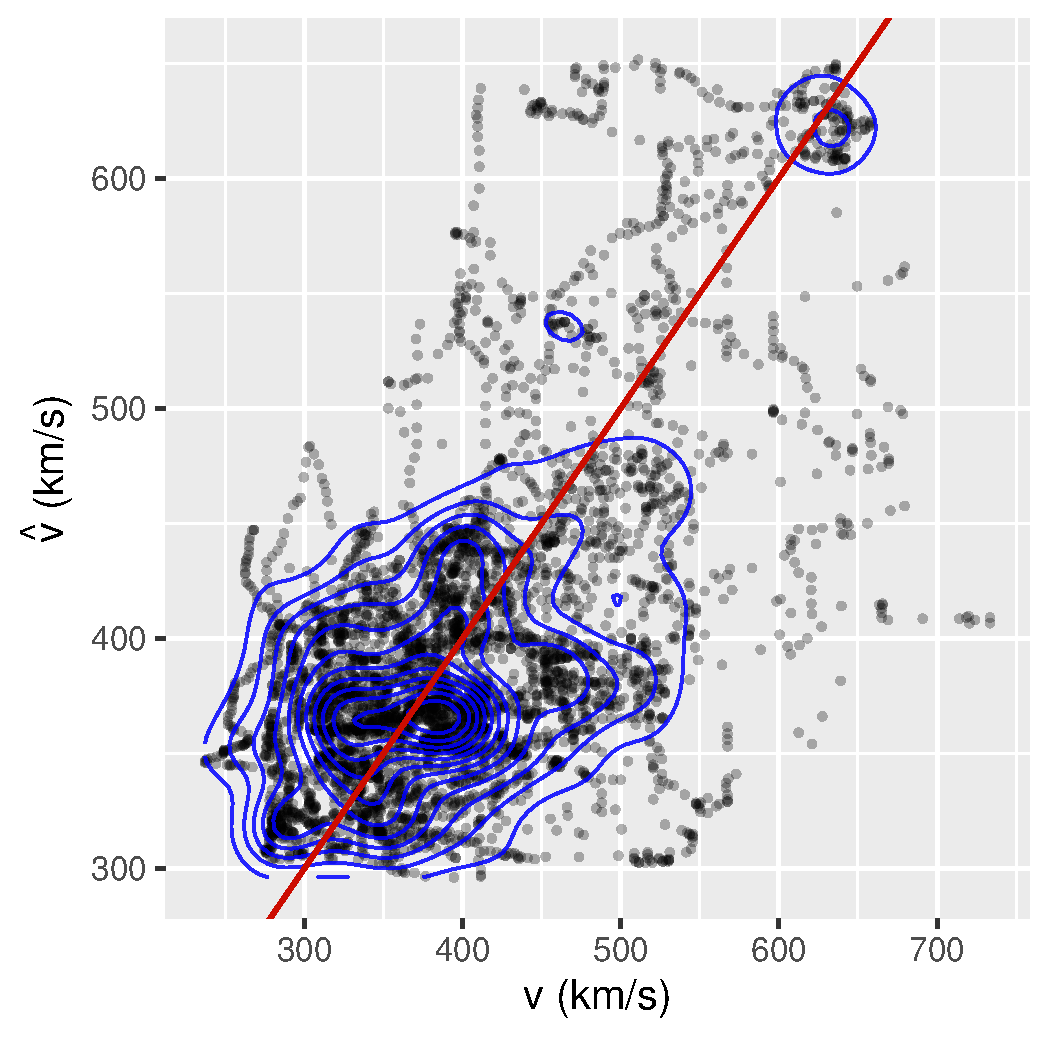
\includegraphics[width=0.4\textwidth]{figures/test_scatter_v}
  \caption{Predicted vs Actual Solar Wind Speed} 
  \label{fig:sw_preds}
\end{figure}

Concerning the solar wind problem, \XX\ finds an operational timelag relationship, with a significantly improved RMSE compared to the vanilla approach (uniform time lag distribution). It is however outperformed by the median time lag based predictor, except for the MAE. This fact is interpreted as the \XX\ model is penalized 
by large rare errors, associated to high speed solar wind (which corresponds to rare events). As usual in real world problems, these experiments raise the question of the quality and representativity of the selected data. Specifically, the geomagnetic phenomenon under consideration is known to be non-stationary \citep{nonstationarysolarwind}, following a 12 year cycle. A first perspective for improving the results thus consists of gathering data from at least one entire solar cycle. 
%The statistic of the time lag is stationary wrt m (only the norm of $x$ is involved); 
%not all the solar cycle; 12 years; more side information; 
%noise is not Gaussian;
%On the real-world problem of the solar wind prediction, \XX\ is dominated by the current best state of the art, intensively using domain theory XXXXXXXXXXXXX. 
The \XX\ results, as displayed on Fig. \ref{fig:sw_preds}, nevertheless shows an encouraging correlation between the predicted and the observed solar wind


\section{Discussion and perspectives}
The contribution of the paper is twofold. Firstly, we define a new ML setting, motivated by an important scientific and practical problem from the domain of space weather, emphasizing that this real-world problem is open for over two decades. This ML setting, called Dynamic Time Lag Regression, is concerned with the inference of lagged causal relationships between time series. 

Secondly, the proposed \XX\ formalization supports the definition of a nested inference procedure, relying on a saddle point optimization process. A closed form analysis of the stability of the inferred model under simplifying assumptions has been conducted, 
yielding a practical alternate optimization formulation, implemented in the \XX\ algorithm. 
The approach demonstrates its merits with some proofs of concept on synthetic problems considering time lag models with diverse complexity. The application on our motivating real-world problem shows the potential of the approach, considering that the \XX\ model involves no domain knowledge in the pre-processing of the data or in the sought prediction model. From an applicative perspective, a next step toward improving the predictive performances will consist of enriching the data sources and the description of the cause series $x_m$.
%, e.g. augmenting the FTE data set with other solar data sources. Importantly, 

On the methodological side, the longer term research perspective consists of extending the proposed nested inference procedure and integrating the model selection step within the inference architecture; the challenge is to provide the algorithm with the means of assessing online the stability and/or the degeneracy of the learning trajectory. 
%Acknowledgement:
%One of the authors (B.P.) wishes to acknowledge Dr. X. P. Zhao for making the CSSS model 
%available to her and the many discussions.



%\bibliographystyle{plainnat}
%\bibliography{references}
